\documentclass[12pt,a4paper]{extarticle} 
%\usepackage{unicode-math}
\usepackage{amsmath,amsfonts,amssymb,amsthm,graphicx,xcolor,natbib,booktabs,tabularx}
%\usepackage[paperwidth=126mm, paperheight=96mm, top=5mm, bottom=5mm, right=5mm, left=5mm]{geometry}
%\usepackage[margin=1cm,footskip=5mm]{geometry}
\usepackage[margin=2cm]{geometry}
\pagenumbering{gobble}

\usepackage[inline]{enumitem}
\usepackage[BoldFont,SlantFont]{xeCJK}  
\xeCJKsetemboldenfactor{2}
\setCJKmainfont{cwTeX Q Yuan Medium}
\newcommand{\ds}{\displaystyle}
\newcommand{\ie}{\;\Longrightarrow\;}
\newcommand{\ifff}{\;\Longleftrightarrow\;}
\newcommand{\orr}{\;\vee\;}
\newcommand{\andd}{\;\wedge\;}
\newcommand{\mi}{\mathrm{i}}
\newcommand{\llt}{\left\langle}
\newcommand{\rgt}{\right\rangle}
\DeclareMathOperator*{\dom}{dom}
\DeclareMathOperator*{\codom}{codom}
\DeclareMathOperator*{\ran}{ran}
\DeclareMathOperator*{\sgn}{sgn}
\DeclareMathOperator*{\degr}{deg}
\newcommand{\floor}[1]{\lfloor #1 \rfloor}
\newcommand{\ceil}[1]{\lceil #1 \rceil}
\newcommand{\proj}[2]{\mathrm{proj}_{\,#2}\,#1}

% figure --> 圖
\renewcommand{\appendixname}{附錄}
\renewcommand{\figurename}{圖}
\renewcommand{\tablename}{表}
\renewcommand{\refname}{參考文獻}

\usepackage{hyperref}
\hypersetup{
    colorlinks,
    linkcolor={red!50!black},
    citecolor={blue!60!black},
    urlcolor={blue!60!black}
}

\theoremstyle{definition}
\newtheorem*{dfn}{定義}
\newtheorem*{prp}{性質}
\newtheorem*{fact}{結論}
\newtheorem*{thm}{定理}
\newtheorem*{ex}{例}
\newtheorem*{sol}{解}
\newtheorem*{prf}{證}
\newtheorem*{rmk}{註}
\newtheorem*{exe}{習題}

\newcommand{\myline}{\noindent\makebox[\linewidth]{\rule{\paperwidth}{0.4pt}}}

\usepackage{pgfplots}
\usetikzlibrary{arrows.meta,angles,quotes,patterns}
% axis style, ticks, etc
\pgfplotsset{every axis/.append style={
                   label style={font=\fontsize{4}{4}\selectfont},
                   tick label style={font=\fontsize{4}{4}\selectfont}  
               },
            }
\renewcommand\tabularxcolumn[1]{m{#1}}

%%%%%%%%%%%%%%%%%%%%%%%%%%%%%%%%%%%%%%%%%%%%%%%%%%%%%%%%%%%%%%%%%%%%%

\usepackage{multicol}
\usepackage{ifthen}
\tikzstyle{vertex}=[shape=circle, minimum size=2mm, inner sep=0, fill]
\tikzstyle{opendot}=[shape=circle, minimum size=2mm, inner sep=0, fill=white, draw]
\newcommand{\myaxis}[7][help lines]{%[formatting of lines]{xlabel}{xleft}{xright}{ylabel}{yleft}{yright}
	\ifthenelse{\lengthtest{#3 pt=0 pt}}{}{
		\draw[ <-,#1] (-#3,0)--(0,0);
		}
	\ifthenelse{\lengthtest{#4 pt=0 pt}}{
		\draw[#1] (0,0)node[right]{$#2$};}{
		\draw[ ->,#1] (0,0)--(#4,0)node[right]{$#2$};
		}
	\ifthenelse{\lengthtest{#6 pt= 0 pt}}{
		}{
		\draw[ <-,#1] (0,-#6)--(0,0);}
	\ifthenelse{\lengthtest{#7 pt= 0 pt}}{
		\draw[#1] (0,0)node[above]{$#5$};
		}{
		\draw[ ->,#1] (0,0)--(0,#7)node[above]{$#5$};}
}

% colorblind-friendly palette
% mixed colours: CB sees contrasting grays
\definecolor{M1}{RGB}{0,0,0}
\definecolor{M2}{RGB}{0,73,73}
\definecolor{M3}{RGB}{0,146,146}
\definecolor{M4}{RGB}{255,109,182}
\definecolor{M5}{RGB}{255,182,119}
% cool colours: CB sees contrasting blues
\definecolor{C1}{RGB}{73,0,146}
\definecolor{C2}{RGB}{0,109,219}
\definecolor{C3}{RGB}{182,109,255}
\definecolor{C4}{RGB}{109,182,255}
\definecolor{C5}{RGB}{182,219,255}
% warm colours: CB sees contrasting yellow
\definecolor{W1}{RGB}{146,0,0}
\definecolor{W2}{RGB}{146,73,0}
\definecolor{W3}{RGB}{219,209,0}
\definecolor{W4}{RGB}{36,255,36}
\definecolor{W5}{RGB}{255,255,109}

%%%%%%%%%%%%%%%%%%%%%%%%%%%%%%%%%%%%%%%%%%%%%%%%%%%%%%%%%%%%%
% from clp3

\newcommand{\vr}{\mathbf{r}}
\newcommand{\vR}{\mathbf{R}}
\newcommand{\vv}{\mathbf{v}}
\newcommand{\va}{\mathbf{a}}
\newcommand{\vb}{\mathbf{b}}
\newcommand{\vc}{\mathbf{c}}
\newcommand{\vd}{\mathbf{d}}
\newcommand{\ve}{\mathbf{e}}
\newcommand{\vC}{\mathbf{C}}
\newcommand{\vp}{\mathbf{p}}
\newcommand{\vn}{\mathbf{n}}
\newcommand{\vu}{\mathbf{u}}
%\newcommand{\vv}{\mathbf{v}}
\newcommand{\vV}{\mathbf{V}}
\newcommand{\vx}{\mathbf{x}}
\newcommand{\vX}{\mathbf{X}}
\newcommand{\vy}{\mathbf{y}}
\newcommand{\vz}{\mathbf{z}}
\newcommand{\vF}{\mathbf{F}}
\newcommand{\vG}{\mathbf{G}}
\newcommand{\vH}{\mathbf{H}}
\newcommand{\vM}{\mathbf{M}}
\newcommand{\vT}{\mathbf{T}}
\newcommand{\vN}{\mathbf{N}}
\newcommand{\vL}{\mathbf{L}}
\newcommand{\vA}{\mathbf{A}}
\newcommand{\vB}{\mathbf{B}}
\newcommand{\vD}{\mathbf{D}}
\newcommand{\vE}{\mathbf{E}}
\newcommand{\vJ}{\mathbf{J}}
\newcommand{\vZero}{\mathbf{0}}
\newcommand{\vPhi}{\mathbf{\Phi}}
\newcommand{\vOmega}{\mathbf{\Omega}}
\newcommand{\vTheta}{\mathbf{\Theta}}
\newcommand{\cA}{\mathcal{A}}
\newcommand{\cB}{\mathcal{B}}
\newcommand{\cM}{\mathcal{M}}
\newcommand{\cO}{\mathcal{O}}
\newcommand{\cR}{\mathcal{R}}
\newcommand{\cS}{\mathcal{S}}
\newcommand{\cT}{\mathcal{T}}
\newcommand{\cU}{\mathcal{U}}
\newcommand{\cV}{\mathcal{V}}
\newcommand{\cW}{\mathcal{W}}
\newcommand{\cX}{\mathcal{X}}

%\newcommand{\hi}{\hat{\mathbf{i}}}
%\newcommand{\hj}{\hat{\mathbf{j}}}
\newcommand{\hi}{\widehat{\pmb{\imath}}}
\newcommand{\hj}{\widehat{\pmb{\jmath}}}
\newcommand{\hk}{\widehat{\mathbf{k}}}
\newcommand{\hn}{\widehat{\mathbf{n}}}
\newcommand{\hr}{\widehat{\mathbf{r}}}
\newcommand{\hvt}{\widehat{\mathbf{t}}}
\newcommand{\hN}{\widehat{\mathbf{N}}}
\newcommand{\vth}{{\pmb{\theta}}}
\newcommand{\vTh}{{\pmb{\Theta}}}
%\newcommand{\vnabla}{\pmb{\nabla}}
\newcommand{\vnabla}{   { \mathchoice{\pmb{\nabla}}
                            {\pmb{\nabla}}
                            {\pmb{\scriptstyle\nabla}}
                            {\pmb{\scriptscriptstyle\nabla}} }   }
\newcommand{\ha}[1]{\mathbf{\hat e}^{(#1)}}

\newcommand{\bbbc}{\mathbb{C}}

\newcommand{\Om}{\Omega}
\newcommand{\om}{\omega}
\newcommand{\vOm}{\pmb{\Omega}}
\newcommand{\svOm}{\pmb{\scriptsize\Omega}}
\newcommand{\al}{\alpha}
\newcommand{\be}{\beta}
\newcommand{\de}{\delta}
\newcommand{\ga}{\gamma}
\newcommand{\ka}{\kappa}
\newcommand{\la}{\lambda}

\newcommand{\cC}{\mathcal{C}}
\newcommand{\bbbone}{\mathbb{1}}

\def\tr{\mathop{\rm tr}}
\newcommand{\Atop}[2]{\genfrac{}{}{0pt}{}{#1}{#2}}

%\newcommand{\pdiff}[2]{ \frac{\partial\hfil#1\hfil}{\partial #2}}
\newcommand{\pdiff}[2]{\frac{\partial #1}{\partial #2}}
\newcommand{\pdifft}[2]{\frac{\partial^2 #1}{\partial #2^2}}
\newcommand{\dblInt}{\iint}
\newcommand{\tripInt}{\iiint}
%\newcommand{\dblInt}{\int\!\!\int}
%\newcommand{\tripInt}{\int\!\!\!\int\!\!\!\int}
%\newcommand{\dblInt}{\mathop{\int\!\!\!\int}}
%\newcommand{\tripInt}{\mathop{\int\!\!\!\int\!\!\!\int}}

\newcommand{\Set}[2]{\big\{ \ #1\ \big|\ #2\ \big\}}
\newcommand{\rhof}{{\rho_{\!{\scriptscriptstyle f}}}}
\newcommand{\rhob}{{\rho_{{\scriptscriptstyle b}}}}

\renewcommand{\neg}{ {\sim} }
\newcommand{\limp}{ {\;\Rightarrow\;} }
\newcommand{\nimp}{ {\;\not\Rightarrow\;} }
\newcommand{\liff}{ {\;\Leftrightarrow\;} }
\newcommand{\niff}{ {\;\not\Leftrightarrow\;} }

\newcommand{\st}{ {\mbox{ s.t. }} }
\newcommand{\es}{ {\varnothing}}
\newcommand{\pow}[1]{ \mathcal{P}\left(#1\right) }
\newcommand{\set}[1]{ \left\{#1\right\} }

\newcommand{\bbbn}{\mathbb{N}}
\newcommand{\bbbr}{\mathbb{R}}
\newcommand{\bbbp}{\mathbb{P}}
\newcommand{\De}{\Delta}
\newcommand{\cD}{\mathcal{D}}
\newcommand{\cP}{\mathcal{P}}
\newcommand{\cI}{\mathcal{I}}
\newcommand{\veps}{\varepsilon}
\newcommand{\dee}[1]{\mathrm{d}#1}

\newcommand{\bdiff}[2]{ \frac{\mathrm{d}}{\mathrm{d}#2} \left( #1 \right)}
\newcommand{\ddiff}[3]{ \frac{\mathrm{d}^#1#2}{\mathrm{d}{#3}^#1}}
\newcommand{\half}{\tfrac{1}{2}}
\newcommand{\diff}[2]{\frac{\mathrm{d} #1}{\mathrm{d} #2}}
\newcommand{\difftwo}[2]{\frac{\mathrm{d^2} #1}{\mathrm{d}{#2}^2}}

%%%%%%%%%%%%%%%%%%%%%%%%%%%%%%%%%%%%%%%%%%%%%%%%%%%%%%%%%%%%%%%%%%%%%

\usepackage{fancyhdr}
\fancypagestyle{firststyle} {
   \fancyhf{}
   \fancyfoot[R]{\footnotesize} %\DTMnow}
   \renewcommand{\headrulewidth}{0pt} 
}
\usepackage{datetime2}

\usepackage{nicefrac}
\newcommand{\eqover}[1]{}

\begin{document}
\title{\texorpdfstring{\vspace{-16mm} 基礎微積分}{基礎微積分}} 
\author{\vspace{-5em}}
\date{\vspace{-5em}}
\maketitle
\thispagestyle{firststyle}

\section*{基本概念}
\subsection*{記號}

\vspace{-5mm}
\begin{table}[!htbp]
  \centering
  \begin{tabular}{lll}
    \toprule
    $\forall$ & 對所有 & for all \\
    $\exists$ & 存在   & there exists \\
    $\exists\,!$ & 存在唯一 & there exists uniquely \\
    $\in$ & 屬於 & belongs to \\
    A $\,\Longrightarrow\,$ B &  若 A 則 B & if A then B \\
    A $\,\Longleftrightarrow\,$ B &  A 等價於 B & A if and only if B \\
    $\infty$ & 無限大 & infinity \\
    $\vee$ & 或 & or \\
    $\wedge$ & 且 & and \\
    $\because$ & 因為 & because \\
    $\therefore$ & 所以 & therefore \\
    \bottomrule
  \end{tabular}
\end{table}

\vspace{-5mm}
\subsection*{數}

\vspace{-5mm}
\begin{table}[!htbp]
  \centering
  \begin{tabular}{llll}
    \toprule
    $\mathbb{N}$ & 自然數 & natural number & $1,\,2,\,3,\,\ldots$ \\
    $\mathbb{Z}$ & 整數   & integer & $\ldots,\,-2,\,-1,\,0,\,1,\,2,\,\ldots$\\
    $\mathbb{Q}$ & 有理數 & rational number & $\ds\frac{p}{q}: \,p,\,q\in\mathbb{Z}$ \\
    $\mathbb{R}$ & 實數 & real number &  \\
    \bottomrule
  \end{tabular}
\end{table}

\vspace{-5mm}
\subsection*{集合}

\vspace{-3mm}
\begin{table}[!htbp]
  \centering
  \begin{tabular}{lll}
    \toprule
    $x\in S$ & $x$ 為集合 $S$ 的元素 &  \\
    $S_1 =\{x_1, x_2, \ldots\}$ & 列舉式   &  \\
    $S_2 =\{ x\,|\, x \text{ 滿足某性質}\}$ & 敘述式 & \\
    $S\cap T$ & $\{x\,|\, x\in S\,\wedge\,x\in T\}$ & 交集 (intersection)    \\
    $S\cup T$ & $\{x\,|\, x\in S\,\vee\,x\in T\}$ & 聯集 (union)    \\
    $S\setminus T$ & $\{x\,|\, x\in S\,\wedge\,x\not\in T\}$ & 差集 (difference)   \\
    $S\times T$ & $\{(x, y)\,|\, x\in S\,\wedge\,y\in T\}$ & 積集 (Cartesian product)  \\
    $\varnothing$ & 空集合 & \\
    $S_1\subset S_2$, $S_2\supset S_1$ & $S_1$ 為 $S_2$ 的真子集合 & \\
    $S_1\subseteq S_2$, $S_2\supseteq S_1$ & $S_1$ 為 $S_2$ 的子集合 & \\
    $\ds\cap_{i=1}^n S_i$ & $S_1\cap S_2\cap\cdots\cap S_n$ &    \\
    $\ds\cup_{i=1}^n S_i$ & $S_1\cup S_2\cup\cdots\cup S_n$ &    \\
    \bottomrule
  \end{tabular}
\end{table}

\vspace{-5mm}
\subsection*{不等式}
\begin{prp}
  令 $a,\;b,\;c\in\mathbb{R}$. 
  \setlength{\columnsep}{-20mm}
  \begin{multicols}{2}
    \begin{enumerate}\setlength\itemsep{0em}
      \item $\ds a < b \ie a + c < b + c$
      \item $\ds a < b, \,c < d \ie a + c < b + d$
      \item $\ds a < b, \,c > 0 \ie a c < b c$
      \item $\ds a < b, \,c < 0 \ie a c > b c$
      \item $\ds0 < a < b \ie \frac{1}{a} > \frac{1}{b}$
    \end{enumerate}
  \end{multicols}
\end{prp}

\begin{ex}
  解下列不等式. 
  \setlength{\columnsep}{-20mm}
  \begin{multicols}{2}
    \begin{enumerate}\setlength\itemsep{0em}
      \item $\ds 2x - 3 < x + 4 < 3 x - 2$
      \item $\ds x^3 > x$
      \item $\ds (2 - x)(1 - x)^2 x^3 \leqslant 0$
      \item $\ds -2 < \frac{2x - 3}{x + 1} < 1$
    \end{enumerate}
  \end{multicols}
\end{ex}

\begin{sol}
  \begin{enumerate}\setlength\itemsep{0em}
    \item[]
    \item $\ds 3 \leqslant x < 7$
    \item $\ds x^3 - x > 0 \ie x(x^2 - 1) > 0 \ie x(x + 1)(x - 1) > 0 \ie x > 1 \vee -1 < x < 0$
    \item $\ds (2 - x)(1 - x)^2 x^3 \leqslant 0 \ie (x - 2)(x - 1)^2 x^3 \geqslant 0 \ie x\geqslant 2 \vee x\leqslant 0\vee x = 1$
    \item $\ds -2 < \frac{2x - 3}{x + 1} < 1 \ie \Big(-2 < \frac{2x - 3}{x + 1}\Big)\wedge\Big(\frac {2x - 3}{x + 1} < 1\Big) \ie \Big(\frac{4x - 1}{x + 1} > 0\Big) \wedge \Big(\frac{x - 4}{x + 1} < 0\Big) \ie \Big(x < -1 \vee x > \frac{1}{4}\Big) \wedge (-1 < x < 4) \ie \frac{1}{4} < x < 4$
  \end{enumerate}
\end{sol}

\subsection*{絕對值}
令 $a\in\mathbb{R}$;  $a$ 的絕對值 (absolute value) $|a|$ 定義為 $\ds|a|=\begin{cases} a & \text{若}\;a\geqslant 0 \\ - a&\text{若}\;a < 0\end{cases}$

\begin{prp}
  若 $a > 0$, 則
  \setlength{\columnsep}{-20mm}
  \begin{multicols}{3}
    \begin{enumerate}\setlength\itemsep{0em}
      \item $\ds |x| = a \ifff x = \pm\,a$
      \item $\ds |x| < a \ifff -a < x < a$
      \item $\ds |x| > a \ifff x < -a \,\vee\, x > a$
    \end{enumerate}
  \end{multicols}
\end{prp}

\begin{prp}
  若 $a, b\in\mathbb{R}$, 則
  \setlength{\columnsep}{-20mm}
  \begin{multicols}{3}
    \begin{enumerate}\setlength\itemsep{0em}
      \item $\ds \sqrt{a^2} = |a|$
      \item $\ds |a b| = |a|\,|b|$
      \item $\ds \Big|\frac{b}{a}\Big| = \frac{|b|}{|a|}$
      \item $\ds |a + b|\leqslant|a| + |b|$
      \item $\ds \big|\,|a| - |b|\,\big|\leqslant|a - b|$
    \end{enumerate}
  \end{multicols}
\end{prp}

\begin{prf}
  \begin{itemize}\setlength\itemsep{0em}
    \item[]
    \item $\ds (|a + b|)^2 = (a + b)^2 = a^2 + 2 a b + b^2 = |a|^2 + 2 a b + |b|^2 \leqslant |a|^2 + 2 |a b| + |b|^2 = |a|^2 + 2 |a|\,|b| + |b|^2 = (|a| + |b|)^2$, 故 $\ds |a + b|\leqslant|a| + |b|$. 
    \item $\ds |a| = |(a - b) + b| \leqslant |a - b| + |b| \ie |a| - |b| \leqslant |a - b|$;  $\ds |b| = |(b - a) + a| \leqslant |b - a| + |a| = |a - b| + |a| \ie |b| - |a| \leqslant |a - b|$.  故 $\ds \big|\,|a| - |b|\,\big|\leqslant|a - b|$. 
  \end{itemize}
\end{prf}

\begin{ex}
  解下列不等式與方程式. 
  \setlength{\columnsep}{-20mm}
  \begin{multicols}{3}
    \begin{enumerate}\setlength\itemsep{0em}
      \item $\ds |5 - 2x| < 3$
      \item $\ds \Big|\frac{2 x - 1}{x + 1}\Big| = 3$
      \item $\ds |x - 1| - |x - 10|\geqslant 5$
    \end{enumerate}
  \end{multicols}
\end{ex}

\begin{sol}
  \begin{enumerate}\setlength\itemsep{0em}
    \item[]
    \item $\ds |5 - 2x| < 3 \ie -3 < 5 - 2x < 3 \ie -8 < -2x < -2 \ie 1 < x < 4$
    \item $\ds \Big|\,\frac{2 x - 1}{x + 1}\,\Big| = 3 \ie \frac{2 x - 1}{x + 1} = 3\,\vee\,\frac{2 x - 1}{x + 1} = -3 \ie x = -4 \,\vee\, x = -\frac{2}{5}$
    \item 當 $x < 1$, $\ds |x - 1| - |x - 10|\geqslant 5 \ie (1 - x) - (10 - x)\geqslant 5 \ie -9 \geqslant 5$, 不合. 當 $1\leqslant x < 10$, $\ds |x - 1| - |x - 10|\geqslant 5 \ie (x - 1) - (10 - x)\geqslant 5 \ie 2 x\geqslant 16 \ie x\geqslant 8$, 則 $8\leqslant x < 10$. 當 $x\geqslant 10$, $\ds |x - 1| - |x - 10|\geqslant 5 \ie (x - 1) - (x - 10)\geqslant 5 \ie 9\geqslant 5$ 恆成立. 綜上, $8\leqslant x$. 
  \end{enumerate}
\end{sol}

\section*{函數}

\begin{dfn}
  \begin{itemize}\setlength\itemsep{0em}
    \item[]
    \item 函數 (function) $f:A\to B$ 是一個對應關係: 對所有 $a\in A$, 存在唯一 $b\in B$, 使得 $f$ 將 $a$ 對應到 $b$. $\ds\forall\,a\in A\;\exists\,!\,b\in B\;(f(a) = b)$.
    \item $A$:  定義域 (domain) ;  $\dom f = A$ \\
          $B$:  對應域 (codomain) ;  $\codom f = B$ \\
          $f(A) = \{f(a)\,|\,a\in A\}\subseteq B$: 值域 (range) ; $\ran f \equiv f(A)$      
  \end{itemize}
\end{dfn}

%\begin{ex}
%  $f(x) = \sqrt{-x^2 + x + 2}$, 求 $\dom f$ 與 $\ran f$. 
%\end{ex}
%
%\begin{sol}
%  由 $-x^2 + x + 2 = -(x + 1)(x - 2)\geqslant 0 \ie (x + 1)(x - 2)\leqslant 0 \ie -1\leqslant x\leqslant 2$, $\dom f = [-1, 2]$. 又 $\ds -x^2 + x + 2 = -\Big(x - \frac{1}{2}\Big)^2 + \frac{4}{9}$, 當 $x\in [-1,2]$ 時, $\ds f(x)\in\Big[0, \sqrt{\frac{4}{9}}\Big] = \Big[0, \frac{2}{3}\Big]$, 故 $\ds\ran f = \Big[0, \frac{2}{3}\Big]$. 
%\end{sol}
%
%\begin{ex}
%  $\ds f(x) = \frac{1}{(x-2)(x-3)}$, 求 $\dom f$ 與 $\ran f$. 
%\end{ex}
%
%\begin{sol}
%  $\dom f = \mathbb{R}\setminus\{2, 3\}$. 令 $\ds y = \frac{1}{(x - 2)(x - 3)} = \frac{1}{x^2 - 5x + 6}\ie x^2 - 5 x + \big(6 - \frac{1}{y}\big) = 0$. 當判別式 $\geqslant 0$ 時有實數解 $\ds\ie 5^2 - 4\big(6 - \frac{1}{y}\big)\geqslant 0 \ie 1 + \frac{4}{y}\geqslant 0 \ie \frac{y + 4}{y}\geqslant 0$, 故 $\ds\ran f = \{y\,|\,y > 0\,\vee\,y\leqslant -4\}$. 
%\end{sol}
%
\subsection*{嵌射與蓋射}
\begin{dfn} 給定函數 $f: A\to B$. 
  \begin{itemize}\setlength\itemsep{0em}
    \item 若 $\forall\,x_1, x_2\in A\,\wedge\,x_1\not=x_2\; (f(x_1)\not=f(x_2))$, 則 $f$ 為嵌射 (one-to-one, injective) . 
    \item 若 $\forall\,b\in B\;\exists\,a\in A\;(f(a) = b)$, 則 $f$ 為蓋射 (onto, surjective) . 
  \end{itemize}
\end{dfn}

%\begin{ex}
%  證明 $f(x) = x^3$ 為嵌射. 
%\end{ex}
%
%\begin{sol}
%  顯然 $\dom f = \mathbb{R}$. 對 $x_1, x_2\in\mathbb{R}$, $x_1^3 - x_2^3 = (x_1 - x_2)(x_1^2 + x_1 x_2 + x_2^2)$. 若 $x_1^3 = x_2^3$, 則 $\ds x_1 - x_2 = 0\ie x_1 = x_2$ $\vee$ $\ds x_1^2 + x_1 x_2 + x_2^2 = 0 \ie \Big(x_1 + \frac{x_2}{2}\Big)^2 + \frac{3x_2^2}{4} = 0 \ie x_2 = x_1 = 0$, 得證.  
%\end{sol}

\section*{函數圖形}

\begin{dfn}
  若 $A$, $B\subseteq\mathbb{R}$, 則函數 $f: A\to B$ 稱為實數值函數 (real-valued function) , 集合 $\{(x, f(x))\,|\,x\in A\}$ 稱為 $f$ 的圖形 (graph) . 
\end{dfn}

\begin{prp}函數 / 圖形判斷法
  \begin{itemize}\setlength\itemsep{0em}
    \item 垂直線判斷法: 函數圖形 $\ifff$ 任一垂直線與其至多交於一點
    \item 水平線判斷法: 嵌射圖形 $\ifff$ 任一水平線與其至多交於一點
  \end{itemize}
\end{prp}

\section*{函數特性}
\subsection*{奇偶性}
\begin{dfn} 給定實數值函數 $f$: 
  \begin{itemize}\setlength\itemsep{0em}
    \item 若 $\forall x\in\dom f$, $f(-x) = f(x)$, 則 $f$ 為偶函數 (even function) . 
    \item 若 $\forall x\in\dom f$, $f(-x) = -f(x)$, 則 $f$ 為奇函數 (odd function) . 
  \end{itemize}
\end{dfn}

\section*{反函數}

\begin{dfn}
  若函數 $f$ 為嵌射, 則其反函數 $f^{-1}:\ran f\to\dom f$ 定義為 $f^{-1}(b) = a \ifff f(a) = b$, 其中 $a\in\dom f$, $b\in\ran f$. 
\end{dfn}

\begin{prp} 反函數常用規則. 
  \setlength{\columnsep}{-0mm}
  \begin{multicols}{2}
    \begin{enumerate}\setlength\itemsep{0em}
      \item $f^{-1}(y) = x \ifff f(x) = y$
      \item $\dom f^{-1} = \ran f$, $\ran f^{-1} = \dom f$
      \item $\ds f^{-1}(x) \not= \frac{1}{f(x)} = (f(x))^{-1}$
      \item $(f^{-1}\circ f)(x) = x$, $\forall\,x\in\dom f$
      \item $(f\circ f^{-1})(y) = y$, $\forall\,y\in\dom f^{-1} = \ran f$
      \item $y = f(x)$ 與 $y = f^{-1}(x)$ 之圖形對 $y = x$ 對稱. 
      \item 若 $f$ 為嚴格遞增或嚴格遞減函數, 則 $f$ 為嵌射 $\ie$ 存在 $f^{-1}$. 
    \end{enumerate}
  \end{multicols}
\end{prp}

\begin{ex} 求反函數. 
  %\setlength{\columnsep}{20mm}
  %\begin{multicols}{2}
    \begin{enumerate}\setlength\itemsep{0em}
      \item 求 $f(x) = x^3 + 2$ 的反函數. 
      \item 求 $f(x) = x^2$, $x\geqslant 0$ 與 $x\leqslant 0$ 的反函數.
      \item 求 $\ds f(x) = \frac{1 + 9 x}{4 - x}$, $x < 4$ 的反函數. 
    \end{enumerate}
  %\end{multicols}
\end{ex}

\begin{sol} 
  \begin{enumerate}\setlength\itemsep{0em}
    \item[]
    \item $y = x^3 + 2$; $x\longleftrightarrow y$: $x = y^3 + 2 \ie y^3 = x - 2 \ie y = \sqrt[3]{x - 2} \ie f^{-1}(x) = \sqrt[3]{x - 2}$.  
    \item $y = x^2$, $x\geqslant 0$;  $x\longleftrightarrow y$: $x = y^2 \ie y^2 = x \ie y = \sqrt{x} \ie f^{-1}(x) = \sqrt{x}$; $f^{-1}:[0, \infty)\to [0, \infty)$. \\$y = x^2$, $x\leqslant 0$;  $x\longleftrightarrow y$: $x = y^2 \ie y^2 = x \ie y = -\sqrt{x} \ie f^{-1}(x) = -\sqrt{x}$; $f^{-1}:[0, \infty)\to (-\infty, 0]$. 
    \item $\ds f(x) = \frac{1 + 9x}{4 - x} \ie y = \frac{1 + 9x}{4 - x}$; $x\longleftrightarrow y$: $\ds x = \frac{1 + 9 y}{4 - y} \ie y = \frac{4 x - 1}{x + 9} \ie f^{-1}(x) = \frac{4 x - 1}{x + 9}$. 檢驗: $\ds (f^{-1}\circ f)(x) = f^{-1}(f(x)) = \frac{4\cdot\frac{1 + 9x}{4 - x} - 1}{\frac{1 + 9x}{4 - x} + 9} = \frac{\frac{4 + 36 x - 4 + x}{4 - x}}{\frac{1 + 9x + 36 - 9x}{4 - x}} = \frac{37 x}{37} = x$; $\ds(f\circ f^{-1})(x) = f(f^{-1}(x)) = \frac{1 + 9\cdot\frac{4x - 1}{x + 9}}{4 - \frac{4 x - 1}{x + 9}} = \frac{\frac{x + 9 + 36 x - 9}{x + 9}}{\frac{4 x + 36 - 4x + 1}{x + 9}} = \frac{37x}{37} = x$. 
  \end{enumerate}
\end{sol}

\section*{指數函數}

$y = f(x) = a^x$, $a > 0\,\wedge a\not=1$. 

\begin{figure}[!htbp]
  \centering
  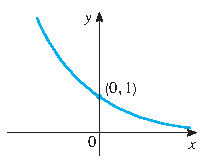
\includegraphics[scale=1.34,page=1]{fig/power.pdf}\qquad\qquad
  \includegraphics[scale=1.34,page=2]{fig/power.pdf}
  \caption{$y = a^x$: 圖左 $0 < a < 1$, 圖右 $a > 1$}
\end{figure}

\begin{prp} 若 $a$, $b > 0$, $x$, $y\in\mathbb{R}$, 則
  \setlength{\columnsep}{-0mm}
  \begin{multicols}{3}
    \begin{itemize}\setlength\itemsep{0em}
      \item $\ds a^x\cdot a^y = a^{x + y}$
      \item $\ds a^{-x} = \frac{1}{a^x}$
      \item $\ds\frac{a^x}{a^y} = a^{x - y}$
      \item $\ds (a^x)^y = a^{xy} = (a^y)^x$
      \item $\ds a^x\cdot b^x = (ab)^x$
      \item $\ds\frac{a^x}{b^x} = \Big(\frac{a}{b}\Big)^x$
    \end{itemize}
  \end{multicols}
\end{prp}

\section*{對數函數}

$y = f(x) = \log_a x$, $a > 0\,\wedge a\not=1$. 

\begin{figure}[!htbp]
  \centering
  \includegraphics[scale=1.,page=3]{fig/power.pdf}\qquad\qquad
  \includegraphics[scale=1.,page=4]{fig/power.pdf}
  \caption{$y = \log_a x$}
\end{figure}

\begin{prp} 給定 $a > 0\,\wedge a\not=1$, $x > 0$, $y\in\mathbb{R}$. 
  \setlength{\columnsep}{-0mm}
  \begin{multicols}{3}
    \begin{itemize}\setlength\itemsep{0em}
      \item $\log_a x = y \ifff a^y = x$
      \item $\ds\log_a a^y = y$
      \item $\ds a^{\log_a x} = x$
    \end{itemize}
  \end{multicols}
\end{prp}

\begin{prp} 給定 $b > 0$, $x > 0$, $a > 0\,\wedge a\not=1$, $c > 0\,\wedge c\not=1$, $r\in\mathbb{R}$. 
  \setlength{\columnsep}{-0mm}
  \begin{multicols}{3}
    \begin{itemize}\setlength\itemsep{0em}
      \item $\log_a b\,x = \log_a b + \log_a x$
      %\item $\ds\log_a\frac{b}{x} = \log_a b - \log_a x$
      \item $\ds\log_a x^r = r\log_a x$
      \item $\ds\log_a x = \frac{\log_c x}{\log_c a}$
    \end{itemize}
  \end{multicols}
\end{prp}

\begin{ex} 解下列 $x$ 的方程式與不等式. 
  \setlength{\columnsep}{-5mm}
  \begin{multicols}{3}
    \begin{enumerate}\setlength\itemsep{0em}
      \item $\ds\log_{10} x + \log_{10}(x - 21) = 2$
      \item $\ds\log_2\big(x^2 - 2x - 2\big)\leqslant 0$
      \item $\ds 3^{\log_3 7} - 4^{\log_4 2} = 5^{\log_5 x - \log_5 x^2}$
    \end{enumerate}
  \end{multicols}
\end{ex}

\begin{sol}
  \vspace{-0.5em}
  \begin{enumerate}\setlength\itemsep{0em}
    \item[]
    \item $\ds\log_{10} (x^2 - 21 x) = \log_{10} 10^2 \ie x^2 - 21x - 100 = 0 \ie (x - 25)(x + 4) = 0 \ie x = 25\,\vee\,x = -4$ (不合) . 
    \item $\ds x^2 - 2x - 2 > 0\,\wedge\, x^2 - 2x - 2\leqslant 1 \ie x \in [-1, 1 - \sqrt{3})\cup (1 + \sqrt{3}, 3]$. 
    \item $\ds 7 - 2 = \frac{1}{x} \ie x = \frac{1}{5}$. 
  \end{enumerate}
\end{sol}

\begin{ex}
  證明 $\ds f(x) = \log_2\big(x + \sqrt{x^2 + 1}\big)$ 為奇函數, 並求其反函數. 
\end{ex}

\begin{sol}
  \vspace{-0.5em}
  \begin{itemize}\setlength\itemsep{0em}
    \item[]
    \item $\ds f(-x) = \log_2\big(-x + \sqrt{x^2 + 1}\big) = \log_2\bigg(\frac{\big(\sqrt{x^2 + 1}\big)^2 - x^2}{\sqrt{x^2 + 1} + x}\bigg) = \log_2\bigg(\frac{1}{x + \sqrt{x^2 + 1}}\bigg) = -f(x)$. 
    \item $\ds y = \log_2\big(x + \sqrt{x^2 + 1}\big)$; $x\longleftrightarrow y$: $\ds x = \log_2\big(y + \sqrt{y^2 + 1}\big)\ie 2^x - y = \sqrt{y^2 + 1} \ie 2^{2x} - 2\cdot2^x y + y^2 = y^2 + 1 \ie y = \frac{2^x - 2^{-x}}{2}$. 
  \end{itemize}
\end{sol}

\section*{直觀極限}

\subsection*{畫圖; 兩邊取接近值}

\begin{minipage}{0.23\textwidth}
\begin{align*}
  \lim_{x\to 2}x = 2
\end{align*}
\end{minipage}
\quad
\begin{minipage}{0.77\textwidth}
%\begin{center}
  \begin{tabular}{cccccccc}
    \toprule
    $x$ & 1.9 & 1.99 & 1.999 & $\circ$ & 2.001 & 2.01 & 2.1 \\
    \hline
    \addlinespace[2mm]
    $f(x)$ & 1.9 & 1.99 & 1.999 & $\circ$ & 2.001 & 2.01 & 2.1 \\
    \bottomrule
  \end{tabular}
%\end{center}
\end{minipage}

\vspace{5mm}

\hspace{-7mm}
\begin{minipage}{0.23\textwidth}
\begin{align*}
  \lim_{x\to 2}x^2 = 4
\end{align*}
\end{minipage}
\quad
\begin{minipage}{0.77\textwidth}
%\begin{center}
  \begin{tabular}{cccccccc}
    \toprule
    $x$ & 1.9 & 1.99 & 1.999 & $\circ$ & 2.001 & 2.01 & 2.1 \\
    \hline
    \addlinespace[2mm]
    $f(x)$ & 3.61 & 3.9601 & 3.996 & $\circ$ & 4.004 & 4.040 & 4.41 \\
    \bottomrule
  \end{tabular}
%\end{center}
\end{minipage}

\vspace{5mm}

\hspace{-5mm}
\begin{minipage}{0.18\textwidth}
\begin{align*}
  \lim_{x\to 2}\frac{x - 2}{x^2 + x - 6} = 0.2
\end{align*}
\end{minipage}
\quad
\begin{minipage}{0.85\textwidth}
%\begin{center}
  \begin{tabular}{cccccccc}
    \toprule
    $x$ & 1.9 & 1.99 & 1.999 & $\circ$ & 2.001 & 2.01 & 2.1 \\
    \hline
    \addlinespace[2mm]
    $f(x)$ & 0.20408 & 0.20040 &0.20004 & $\circ$ & 0.19996 & 0.19960 & 0.19608 \\
    \bottomrule
  \end{tabular}
%\end{center}
\end{minipage}

\section*{單側極限, 在無限遠之極限, 無窮極限}

\subsection*{單側極限 (One-Sided Limits) }
\vspace{-10mm}

\begin{figure}[ht]
  \centering
  \begin{tabularx}{0.8\textwidth}{X>{\centering\arraybackslash}X}
    \begin{align*}
      \lim_{x\to2-}g(x) = 3,\qquad\lim_{x\to5-}g(x) = 2 \\
      \lim_{x\to2+}g(x) = 1,\qquad\lim_{x\to5+}g(x) = 2 \\
      \lim_{x\to2}g(x) = \text{DNE},\qquad\lim_{x\to5}g(x) = 2
    \end{align*}
  &  
  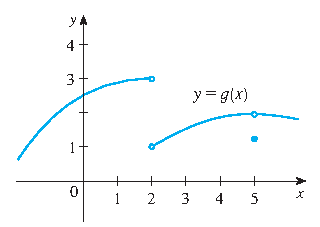
\includegraphics[scale=1.4,page=1]{fig/g.pdf}
 \end{tabularx}
\end{figure}

\vspace{-12mm}

\begin{ex}
  $\ds g(x) = \begin{cases}\sqrt{x - 4} & \text{若 } x > 4 \\ 8 - 2x & \text{若 } x < 4 \end{cases}$, $\ds\lim_{x\to 4}g(x) = 0$. 
\end{ex}

\begin{ex}
  $\ds f(x) = \sqrt{4 - x^2}$, $\ds\lim_{x\to(-2)+}f(x) = 0$, $\ds\lim_{x\to2+}f(x) = \text{DNE}$, $\ds\lim_{x\to2-}f(x) = 0$. 
\end{ex}

\begin{thm}
  若 $F\in\mathbb{R}$, $\ds\lim_{x\to a}f(x) = F$ $\ifff$ $\ds\lim_{x\to a-} f(x) = \ds\lim_{x\to a+} f(x) = F$. 
\end{thm}

\subsection*{在無限遠的極限 (Limits at Infinity) }
\begin{ex}
  \begin{multicols}{2}
    \begin{itemize}\setlength\itemsep{0em}
      \item $\ds\lim_{x\to\infty}\frac{1}{x^\alpha} = 0$, $\alpha > 0$; $\ds\lim_{x\to-\infty}\frac{1}{x^N} = 0$, $\forall\,N\in\mathbb{N}$
      \item $\ds\lim_{x\to\infty}a^x = \infty$, $\ds\lim_{x\to-\infty}a^x = 0$, $\ds\lim_{x\to0-}a^{\frac{1}{x}} = 0$, $\forall\,a > 1$. 
    \end{itemize}
  \end{multicols}
\end{ex}

\subsection*{無窮極限 (Infinite Limits) }
\begin{ex}
  \setlength{\columnsep}{-20mm}
  \begin{multicols}{4}
    \begin{itemize}\setlength\itemsep{0em}
      \item $\ds\lim_{x\to0+}\frac{1}{x} = \infty$
      \item $\ds\lim_{x\to0-}\frac{1}{x} = -\infty$
      \item $\ds\lim_{x\to0}\frac{1}{x} = \text{DNE}$
      \item $\ds\lim_{x\to0}\frac{1}{x^2} = \infty$
    \end{itemize}
  \end{multicols}
\end{ex}

\section*{極限運算}

\begin{thm}[極限四則運算]
  若 $\ds\lim_{x\to a}f(x) = F$, $\ds\lim_{x\to a}g(x) = G$, 則
  \begin{multicols}{2}
    \begin{enumerate}\setlength\itemsep{0em}
      \item $\ds\lim_{x\to a} c = c$, $\ds\lim_{x\to a} x = a$
      \item $\ds\lim_{x\to a} k\,f(x) = k\,F$ 
      \item $\ds\lim_{x\to a} \big(f(x)\pm g(x)\big) = F\pm G$ 
      \item $\ds\lim_{x\to a} \big(f(x)\cdot g(x)\big) = F\cdot G$ 
      \item $\ds\lim_{x\to a} \frac{f(x)}{g(x)} = \frac{F}{G}$, 若 $G\ne 0$
      \item $\ds\lim_{x\to a} \big(f(x)\big)^\alpha = F^\alpha$, 若 $\alpha\in\mathbb{Q}\,\wedge\,F > 0$
    \end{enumerate}
  \end{multicols}
  當 $F$, $G$ 存在 (非為無窮) , 此定理敘述對「單側極限」及「無限遠之極限」均成立. 
\end{thm}

\begin{ex}
  \begin{itemize}\setlength\itemsep{0em}
    \item[]
    \item $\ds\lim_{h\to0}\frac{(2 + h)^2 - 4}{2 h} = \lim_{h\to0}\frac{h^2 + 4h + 4 - 4}{2 h} = \lim_{h\to0}\frac{h^2 + 4h}{2 h} =\lim_{h\to0}\frac{h + 4}{2} = 2$
    \item $\ds\lim_{x\to4}\frac{x^2 - 4x}{x^2 - 16} = \lim_{x\to4}\frac{x(x - 4)}{(x - 4)(x + 4)} = \lim_{x\to4}\frac{x}{x + 4} = \frac{1}{2}$
    \item $\ds\lim_{x\to 2}\frac{x - 2}{x^2 + x - 6} = \lim_{x\to 2}\frac{x - 2}{(x - 2)(x + 3)} = \lim_{x\to2}\frac{1}{x + 3} = \frac{1}{5}$
  \end{itemize}
\end{ex}

\begin{ex}
  求 $\ds\lim_{x\to-1}\frac{\sqrt{x^2 + 8} - 3}{x + 1}$. 
\end{ex}

\begin{sol}
  $\ds\lim_{x\to-1}\frac{\sqrt{x^2 + 8} - 3}{x + 1} = \lim_{x\to-1}\frac{1}{x + 1}\frac{(x^2 + 8) - 3^2}{\sqrt{x^2 + 8} + 3} = \lim_{x\to-1}\frac{1}{x + 1}\frac{x^2 - 1}{\sqrt{x^2 + 8} + 3} \\= \lim_{x\to-1}\frac{1}{x + 1}\frac{(x + 1)(x - 1)}{\sqrt{x^2 + 8} + 3} =\lim_{x\to-1}\frac{x - 1}{\sqrt{x^2 + 8} + 3} = \frac{-2}{\sqrt{1 + 8} + 3} = -\frac{1}{3}$. 
\end{sol}

\begin{ex}
  求 $\ds\lim_{x\to3}\frac{\sqrt{x - 2} - \sqrt{4 - x}}{x - 3}$. 
\end{ex}

\begin{sol}
  $\ds\lim_{x\to3}\frac{\sqrt{x - 2} - \sqrt{4 - x}}{x - 3} = \lim_{x\to3}\frac{1}{x - 3}\frac{(x - 2) - (4 - x)}{\sqrt{x - 2} + \sqrt{4 - x}} = \lim_{x\to3}\frac{1}{x - 3}\frac{2 x - 6}{\sqrt{x - 2} + \sqrt{4 - x}} \\= \lim_{x\to3}2\frac{1}{\sqrt{x - 2} + \sqrt{4 - x}} = \frac{2}{\sqrt{1} + \sqrt{1}} = 1$. 
\end{sol}

\begin{ex}
  $\ds\lim_{x\to\infty}\frac{5x^2 + 8x - 3}{3x^2 + 2} = \lim_{x\to\infty}\frac{5 + \frac{8}{x} - \frac{3}{x^2}}{3 + \frac{2}{x^2}} = \frac{5 + 0 + 0}{3 + 0} = \frac{5}{3} = \lim_{x\to-\infty}\frac{5x^2 + 8x - 3}{3x^2 + 2}$. 
\end{ex}

\begin{ex}
  求 $\ds\lim_{x\to\infty}\big(\sqrt{x^2 + 5x} - \sqrt{x^2 - x}\big)$. 
\end{ex}

\begin{sol}
  $\ds\lim_{x\to\infty}\big(\sqrt{x^2 + 5x} - \sqrt{x^2 - x}\big) = \lim_{x\to\infty}\frac{(x^2 + 5x) - (x^2 - x)}{\sqrt{x^2 + 5x} + \sqrt{x^2 - x}} = \lim_{x\to\infty}\frac{6 x}{\sqrt{x^2\big(1 + \frac{5}{x}\big)} + \sqrt{x^2\big(1 - \frac{1}{x}\big)}} \\ = \lim_{x\to\infty}\frac{6 x}{|x|\sqrt{1 + \frac{5}{x}} + |x|\sqrt{1 - \frac{1}{x}}} = \lim_{x\to\infty}\frac{6 x}{x\sqrt{1 + \frac{5}{x}} + x\sqrt{1 - \frac{1}{x}}} = \lim_{x\to\infty}\frac{6}{\sqrt{1 + \frac{5}{x}} + \sqrt{1 - \frac{1}{x}}} \\= \frac{6}{\sqrt{1 + 0} + \sqrt{1 - 0}} = 3$
\end{sol}

\begin{ex}
  求 $\ds\lim_{x\to-\infty}\frac{3x}{\sqrt{4x^2 + x} - 2x}$. 
\end{ex}

\begin{sol}
  變數變換 $y = -x\ie x=-y$: $\ds\lim_{x\to-\infty}\frac{3x}{\sqrt{4x^2 + x} - 2x} = \lim_{y\to\infty}\frac{-3y}{\sqrt{4y^2 - y} + 2y} = \lim_{y\to\infty}\frac{-3y}{\sqrt{y^2\big(4 - \frac{1}{y}\big)} + 2y} = \lim_{y\to\infty}\frac{-3y}{|y|\sqrt{4 - \frac{1}{y}} + 2y} =\lim_{y\to\infty}\frac{-3y}{y\sqrt{4 - \frac{1}{y}} + 2y} =\lim_{y\to\infty}\frac{-3}{\sqrt{4 - \frac{1}{y}} + 2} = -\frac{3}{4}$. 
\end{sol}

\section*{連續性}

\begin{dfn} 給定 $f$, $a\in\dom f$. 
  \begin{itemize}\setlength\itemsep{0em}
    \item 若 $\ds\lim_{x\to a} f(x)$ 存在且 $\ds f(a)=\lim_{x\to a}f(x)$, 則稱 $f$ 在 $a$ \emph{連續}.  
    \item 若 $\ds\lim_{x\to a+} f(x)$ 存在且 $\ds f(a)=\lim_{x\to a+}f(x)$, 則稱 $f$ 在 $a$ \emph{左連續}.  
    \item 若 $\ds\lim_{x\to a-} f(x)$ 存在且 $\ds f(a)=\lim_{x\to a-}f(x)$, 則稱 $f$ 在 $a$ \emph{右連續}.  
  \end{itemize}
  $f(x)$ 在 $a$ 連續 $\ifff$ $\ds\lim_{x\to a}f(x) = f\big(\lim_{x\to a}x\big)$
\end{dfn}

\begin{dfn}[端點連續性]
  給定 $f$, $\dom f = [a, b]$.  
  \begin{multicols}{2}
    \begin{itemize}\setlength\itemsep{0em}
      \item 若 $f$ 在 $b$ 左連續, 則稱 $f$ 在 $b$ 連續.  
      \item 若 $f$ 在 $a$ 右連續, 則稱 $f$ 在 $a$ 連續.  
    \end{itemize}
  \end{multicols}
\end{dfn}

\begin{dfn}[連續函數] 
  \begin{itemize}\setlength\itemsep{0em}
    \item[]
    \item 若 $f$ 在區間 $I$ 之每一點均連續, 則稱 $f$ 在 $I$ 連續.  
    \item 若 $f$ 在 $\dom f$ 之每一點均連續, 則稱 $f$ 為\emph{連續函數}.  
  \end{itemize}
\end{dfn}

\begin{thm}[五則運算仍連續]
  \begin{itemize}\setlength\itemsep{0em}
    \item[] 
    \item 若 $f$, $g$ 在 $a$ 連續, 則 $f\pm g$, $f\cdot g$, $k f$, $f^\alpha$, $\ds\frac{f}{g}$ (若 $g(a)\ne 0$) 均在 $a$ 連續. 
    \item 若 $f$ 在 $a$ 連續, 且 $g$ 在 $f(a)$ 連續, 則 $g\circ f$ 在 $a$ 連續. 
  \end{itemize}
\end{thm}

\begin{rmk}
  多項式, 指數, 對數函數及其五則運算之組合均為連續函數. 
\end{rmk}

\begin{ex}
  若 $\ds f(x) = \begin{cases}x + 2 & \text{當 }\; x < a \\ x^2 & \text{當 }\; x\geqslant a\end{cases}$ 為連續函數, 求 $a$. 
\end{ex}

\begin{sol}
  若 $f$ 為連續函數, 則 $f$ 在 $a$ 連續 $\ds\ie \lim_{x\to a-}f(x) = \lim_{x\to a+} f(x) \ie a + 2 = a^2 \ie a = -1\,\vee\, a = 2$. 
\end{sol}

\begin{ex}
  若 $\ds f(x) = \begin{cases}\frac{x^2 - 4}{x - 2} & \text{當 }\; x < 2 \\ a x^2 - b x + 3 & \text{當 }\; 2 \leqslant x < 3 \\ 2 x - a + b & \text{當 }\; x \geqslant 3 \end{cases}$ 為連續函數, 求 $a$, $b$. 
\end{ex}

\begin{sol}
  若 $f$ 為連續函數, 則 $f$ 在 $2$, $3$ 均連續 $\ds\ie \big(\lim_{x\to 2-}f(x) = \lim_{x\to 2+} f(x)\big) \,\wedge\, \big(\lim_{x\to 3-}f(x) = \lim_{x\to 3+} f(x)\big)\ie (4 = 4a - 2b + 3)\,\wedge\, (9a - 3b + 3 = 6 - a + b)\ie a = \frac{1}{2},\,\,b = \frac{1}{2}$. 
\end{sol}

\section*{導數與導函數}

\begin{minipage}{0.4\textwidth}
  %\begin{figure}[!htbp]
  %  \centering
  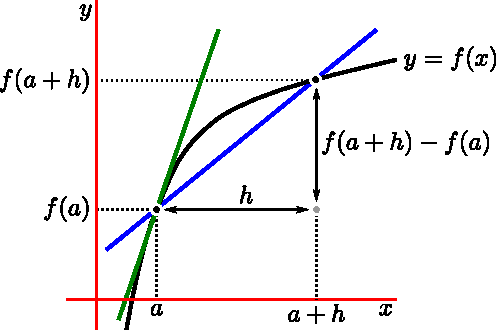
\includegraphics[scale=0.8,page=1]{fig/tangentA.pdf}
  %\end{figure}
\end{minipage}
\quad
\begin{minipage}{0.6\textwidth}
  \begin{dfn}
    給定 $f(x)$, $a\in\dom f$. $f$ 在 $a$ 的導數 (derivative) $f'(a)$ 定義為 $$f'(a) = \lim_{h\to 0}\frac{f(a + h) - f(a)}{h}$$ 若 $f'(a)$ 存在, 則稱 $f$ 在 $a$ 可微(分)(differentiable). \\  
    $f$ 的導函數 $f'(x)$ 定義為 $$f'(x) = \lim_{h\to 0}\frac{f(x + h) - f(x)}{h}$$ 
    %\end{itemize}
  \end{dfn}
\end{minipage}

\begin{rmk}
  \begin{itemize}\setlength\itemsep{0em}
    \item[]
    \item 求導函數之過程稱為微分 (differentiation) : 求 $f'(x)$ $\ifff$ $f(x)$ (對 $x$) 微分
    \item 給定 $y = f(x)$, 其導函數可記為 $\ds f'(x) = f' = y' = \frac{\text{d}y}{\text{d}x} = \frac{\text{d}f}{\text{d}x} = \frac{\text{d}}{\text{d}x} f(x) = Df(x) = D_x f(x)$. 
    \item $f$ 在 $a$ 的導數可記為 $\ds f'(a) = \Big.\frac{\text{d}y}{\text{d}x}\Big|_{x = a}$.  
  \end{itemize}
\end{rmk}

\begin{ex}
  求以下 $f(x)$ 之導函數 $f'(x)$。
  \setlength{\columnsep}{-7mm}
  \begin{multicols}{6}
    \begin{enumerate}\setlength\itemsep{0em}
      \item $f(x) = x$ 
      \item $f(x) = x^2$
      \item $f(x) = x^4$
      \item $f(x) = \frac{1}{x}$ 
      \item $f(x) = \frac{1}{x^5}$
      \item $f(x) = \frac{1}{x^2 + 3}$
    \end{enumerate}
  \end{multicols}
\end{ex}

\begin{sol}
  \begin{enumerate}\setlength\itemsep{0em}
    \item[]
    \item $\ds f'(x) = \lim_{h\to 0}\frac{(x + h) - x}{h} = \lim_{h\to 0}\frac{h}{h} = \lim_{h\to 0}\,1 = 1$. 
    \item $\ds f'(x) = \lim_{h\to 0}\frac{(x + h)^2 - x^2}{h} = \lim_{h\to 0}\frac{2 x h + h^2}{h} = \lim_{h\to 0}\,(2x + h) = 2x$. 
    \item $\ds f'(x) = \lim_{h\to 0}\frac{(x + h)^4 - x^4}{h} = \lim_{h\to 0}\frac{4 x^3 h + 6x^2 h^2 + 4 x h^3 + h^4}{h} = \lim_{h\to 0}\,(4x^3 + 6x^2 h + 4 x h^2 + h^3) = 4x^3$. 
    \item $\ds f'(x) = \lim_{h\to 0}\frac{\frac{1}{x + h} - \frac{1}{x}}{h} = \lim_{h\to 0}\frac{x - (x + h)}{h\,(x + h)\,x} = \lim_{h\to 0}\frac{-h}{h\,(x + h)\,x} = \lim_{h\to 0}\frac{-1}{(x + h)\,x} = \frac{-1}{x^2} = (-1)\,x^{-2}$. 
    \item $\ds f'(x) = \lim_{h\to 0}\frac{\frac{1}{(x + h)^5} - \frac{1}{x^5}}{h} = \lim_{h\to 0}\frac{x^5 - (x + h)^5}{h\,(x + h)^5\,x^5} \\ = \lim_{h\to 0}\frac{(-h)(x^4 + x^3(x + h) + x^2(x + h)^2 + x^3(x + h) + (x + h)^4)}{h\,(x + h)^5\,x^5}\\ = \lim_{h\to 0}\frac{-(x^4 + x^3(x + h) + x^2(x + h)^2 + x^3(x + h) + (x + h)^4)}{(x + h)^5\,x^5} = \frac{-5x^4}{x^{10}} = \frac{-5}{x^6} = (-5)\,x^{-6}$. 
   \item $\ds f'(x) = \lim_{h\to 0}\frac{\frac{1}{(x + h)^2 + 3} - \frac{1}{x^2 + 3}}{h} = \lim_{h\to 0}\frac{(x^2 + 3) - ((x + h)^2 + 3)}{h\,((x + h)^2 + 3)\,(x^2 + 3)} = \lim_{h\to 0}\frac{(2x + h)\,(-h)}{h\,((x + h)^2 + 3)\,(x^2 + 3)} \\ = \lim_{h\to 0}\frac{-(2x + h)}{((x + h)^2 + 3)(x^2 + 3)} = \frac{-2x}{(x^2 + 3)^2}$. 
  \end{enumerate}
\end{sol}

\begin{fact}
  $x^\alpha$ ($\alpha\in\mathbb{R}$) 之導函數為 $\alpha\,x^{\alpha - 1}$. 
\end{fact}

\begin{dfn}
  若 $f$ 在 $(a, b)$ 上每一點均有導數, 則稱 $f$ 在 $(a, b)$ 可微 (分) . 
\end{dfn}

\begin{thm}
  若 $f$ 在 $a$ 可微, 則 $f$ 在 $a$ 連續. 
\end{thm}

\section*{微分規則}

\begin{thm}[四則運算] 令 $f$, $g$ 可微, $c\in\mathbb{R}$. 則
  \setlength{\columnsep}{-0mm}
  \begin{multicols}{3}
    \begin{enumerate}\setlength\itemsep{0em}
      \item $\ds (c)' = 0$
      \item $\ds (c\,f)' = c\,f'$
      \item $\ds (f\pm g)' = f'\pm g'$
      \item $\ds (f\cdot g)' = f'\cdot g + f\cdot g'$
      \item $\ds \Big(\frac{f}{g}\Big)' = \frac{f'\cdot g - f\cdot g'}{g^2}$
    \end{enumerate}
  \end{multicols}
\end{thm}

\begin{ex} 求導函數。
  \begin{multicols}{3}
    \begin{enumerate}\setlength\itemsep{0em}
      \item $x^5$
      \item $\frac{x - 1}{x + 1}$
      \item $\frac{1}{x^2 + 3}$
    \end{enumerate}
  \end{multicols}
\end{ex}

\begin{sol}
  \begin{enumerate}\setlength\itemsep{0em}
    \item[]
    \item $\ds (x^5)' = (x \cdot x^2 \cdot x^2)' = (x)'\cdot x^2 \cdot x^2 + x\cdot(x^2)'\cdot x^2 + x\cdot x^2\cdot(x^2)' = x^4 + x\cdot(2x)\cdot x^2 + x^3\cdot(2x) = 5 x^4$
    \item $\ds\Big(\frac{x - 1}{x + 1}\Big)' = \frac{(x + 1)\cdot(x - 1)' - (x - 1)\cdot(x + 1)'}{(x + 1)^2} = \frac{2}{(x + 1)^2}$ 
    \item $\ds\Big(\frac{1}{x^2 + 3}\Big)' = \frac{(x^2 + 3)\cdot(1)' - 1\cdot(x^2 + 3)'}{(x^2 + 3)^2} = \frac{-2x}{(x^2 + 3)^2}$
  \end{enumerate}
\end{sol}

\begin{thm}[鏈鎖律 (chain rule) ]
  若 $f(u)$ 在 $u = g(x)$ 可微, $g(x)$ 在 $x$ 可微, 則 $f\circ g$ 在 $x$ 可微: 
  \begin{align*}
    (f\circ g)'(x)\,\equiv\,(f(g(x)))' = f'(g(x))\cdot g'(x)
  \end{align*}
\end{thm}

\begin{ex} 求導函數.
  \begin{multicols}{4}
    \begin{enumerate}\setlength\itemsep{0em}
      \item $(x^3 - 1)^{2023}$
      \item $\sqrt{x^2 + 1}$
      \item $\frac{1}{x^2 + 3}$
      \item $\sqrt{\frac{x - 1}{x + 1}}$
    \end{enumerate}
  \end{multicols}
\end{ex}

\begin{sol}
  \begin{enumerate}\setlength\itemsep{0em}
    \item[]
    \item 令 $\ds f(u) = u^{2023}$, $g(x) = x^3 - 1$, 則 $\ds f'(u) = 2023\,u^{2022}$, $\ds(x^3 - 1)^{2023} = f(g(x))$. \\由鏈鎖律 $\ds((x^3 - 1)^{2023})' = (f(g(x)))' = f'(g(x))\cdot g'(x) = 2023\cdot(x^3 - 1)^{2022}\cdot(3x^2)$. 
    \item 令 $\ds f(u) = \sqrt{u} = u^{\frac{1}{2}}$, $g(x) = x^2 + 1$, 則 $\ds f'(u) = \frac{1}{2\sqrt{u}}$, $\ds\sqrt{x^2 + 1} = f(g(x))$. \\由鏈鎖律 $\ds (\sqrt{x^2 + 1})' = (f(g(x)))' = f'(g(x))\cdot g'(x) = \frac{1}{2\sqrt{x^2 + 1}}\cdot(2x) = \frac{x}{\sqrt{x^2 + 1}}$. 
    \item 令 $\ds f(u) = \frac{1}{u}$, $g(x) = x^2 + 3$, 則 $\ds f'(u) = \frac{-1}{u^2}$, $\ds\frac{1}{x^2 + 3} = f(g(x))$. \\由鏈鎖律 $\ds\Big(\frac{1}{x^2 + 3}\Big)' = (f(g(x)))' = f'(g(x))\cdot g'(x) = \frac{-1}{(x^2 + 3)^2}\cdot(x^2 + 3)' = \frac{-2x}{(x^2 + 3)^2}$. 
    \item 令 $\ds f(u) = \sqrt{u}$, $\ds g(x) = \frac{x - 1}{x + 1}$, 則 $\ds f'(u) = \frac{1}{2\sqrt{u}}$, $\ds\sqrt{\frac{x - 1}{x + 1}} = f(g(x))$. \\由鏈鎖律 $\ds\bigg(\sqrt{\frac{x - 1}{x + 1}}\bigg)' = (f(g(x)))' = f'(g(x))\cdot g'(x) = \frac{1}{2\sqrt{\frac{x - 1}{x + 1}}}\cdot\Big(\frac{x - 1}{x + 1}\Big)' = \frac{1}{2\sqrt{\frac{x - 1}{x + 1}}}\frac{2}{(x + 1)^2} = \frac{1}{\sqrt{(x - 1)(x + 1)^3}}$. 
  \end{enumerate}
\end{sol}

\begin{fact}
  若 $f(g(x)) = x$, 則等式兩邊對 $x$ 微分 $\ie$ $\ds(f(g(x)))' = 1$ $\ie$ $\ds f'(g(x))\cdot g'(x) = 1$ $\ie$ $\ds g'(x) = \frac{1}{f'(g(x))}$.   
\end{fact}

\section*{自然指數, 對數與微分}

\begin{dfn}[自然指數 $e$ 與 $e^x$ 微分]
  \begin{itemize}\setlength\itemsep{0em}
    \item[]
    \item 給定 $a > 0$, 求 $f(x) = a^x$ 之導函數
    \item $\ds\diff{f}{x}=\lim_{h \to 0} \frac{f(x+h) - f(x)}{h} = \lim_{h \to 0} \frac{a^{x+h} - a^x}{h} = \lim_{h \to 0} a^x \cdot \frac{a^{h} - 1}{h} = a^x \cdot \lim_{h \to 0} \frac{a^{h} - 1}{h}$
    \item 令 $\ds C(a) = \lim_{h \to 0} \frac{a^{h} - 1}{h}$, 則 $\ds\diff{}{x}a^x =  C(a)\cdot a^x$
    \item 觀察: $C(a)$ 隨 $a$ 遞增; 對於某個介於 $2$, $3$ 間的 $a$, $C(a) = 1$. 
      \begin{table}[!htbp]
        \centering
        \begin{tabular}{cccccccc}
        \toprule
        $h$ & $10^{-1}$ & $10^{-2}$ & $10^{-3}$ & $10^{-4}$ & $10^{-5}$ & $10^{-6}$ & $10^{-7}$ \\
        \midrule
        \addlinespace[1mm]
        $\ds\frac{2^h-1}{h}$ & 0.7177 & 0.6956 & 0.6934 & 0.6932 & 0.6931 & 0.6931 & 0.6931 \\
        \addlinespace[1mm]
        $\ds\frac{3^h-1}{h}$ & 1.1612 & 1.1047 & 1.0992 & 1.0987 & 1.0986 & 1.0986 & 1.0986 \\
        \addlinespace[1mm]
        $\ds\frac{5^h-1}{h}$ & 1.7462 & 1.6225 & 1.6107 & 1.6096 & 1.6095 & 1.6094 & 1.6094 \\
        \addlinespace[1mm]
        $\ds\frac{10^h-1}{h}$ & 2.5893 & 2.3293 & 2.3052 & 2.3028 & 2.3026 & 2.3026 & 2.3026 \\ 
        \addlinespace[1mm]
        \bottomrule
        \end{tabular}
      \end{table}
    \item 定義 $\ds C(e) = 1 \ie \lim_{h\to 0}\frac{e^h - 1}{h} = 1$, 則 $\ds\diff{}{x}e^x = C(e)\cdot e^x \ie (e^x)' = e^x$. $\ds\;\ln x \equiv\log_e x$
  \end{itemize}
\end{dfn}

\begin{prp}
  $\ds\;(\ln |x|)' = \frac{1}{x}$. 
\end{prp}

\begin{sol}
  \begin{itemize}
    \item[]
    \item 若 $x > 0$, $\ln |x| = \ln x$ 且 $\ds e^{\ln x} = x$. 令 $f(u) = e^u$, $g(x) = \ln|x| = \ln x$, 則 $\ds f'(u) = e^u$, $\ds f(g(x)) = x$; 故 $\ds g'(x) = \frac{1}{f'(g(x))}\ie (\ln|x|)' = (\ln x)' = \frac{1}{e^{\ln x}} = \frac{1}{x}$. 
    \item 若 $x < 0$, $\ln |x| = \ln(-x)$ 且 $\ds e^{\ln(-x)} = -x$. 令 $f(u) = e^u$, $g(x) = \ln|x| = \ln(-x)$, 則 $\ds f'(u) = e^u$, $\ds f(g(x)) = -x$; 故 $\ds g'(x) = \frac{-1}{f'(g(x))}\ie (\ln|x|)' = (\ln(-x))' = \frac{-1}{e^{\ln(-x)}} = \frac{1}{x}$. 
  \end{itemize}
\end{sol}

\begin{prp}
  $\ds(a^x)' = a^x\cdot\ln a,\;\forall\,a > 0$. 
\end{prp}

\begin{prf}
  $\ds a = e^{\log_e a} \equiv e^{\ln a} \ie a^x = e^{x\ln a}$. 令 $f(u) = e^u$, $g(x) = x\ln a$, 則 $\ds f'(u) = e^u$, $\ds f(g(x)) = e^{x\ln a} = a^x$; 故 $(f(g(x)))' = f'(g(x))\cdot g'(x) = e^{x\ln a}\cdot(x\ln a)' = a^x\cdot\ln a$. 
\end{prf}

\begin{fact}
  $\ds C(a) = \ln a$. 
\end{fact}

\begin{prp}
  $\ds (x^\alpha)' = \alpha\,x^{\alpha - 1}$ ($\alpha\in\mathbb{R}$) 
\end{prp}

\begin{sol}
  $\ds x^\alpha = e^{\ln x^\alpha} = e^{\alpha\ln x}$. 故 $\ds(x^\alpha)' = (e^{\alpha\ln x})' = e^{\alpha\ln x}\cdot\big(\alpha\cdot\frac{1}{x}\big) = x^\alpha\cdot\alpha\cdot\frac{1}{x} = \alpha\,x^{\alpha - 1}$. 
\end{sol}

\begin{thm}[均值定理 (mean-value theorem, MVT) ]
  若 $f(x)$ 在 $[a, b]$ 連續, 在 $(a, b)$ 可微, 則存在 $\ds c\in (a, b)$ 使 $\ds f'(c) = \frac{f(b) - f(a)}{b - a}$. 
\end{thm}
\vspace{-5mm}
\begin{figure}[!htbp]
  \centering
  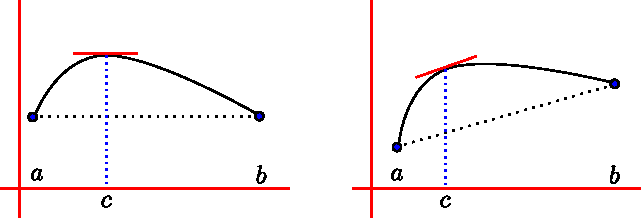
\includegraphics[scale=1,page=1]{fig/rolle_to_mvt.pdf}
\end{figure}

\begin{prp}
  $f(x)$ 在 $[a, b]$ 連續, 在 $(a, b)$ 可微. 若
  %\setlength{\columnsep}{15mm}
  %\begin{multicols}{2}
    \begin{enumerate}\setlength\itemsep{0em}
      \item $\ds\forall\,x\in(a, b)\; f'(x) > 0$, 則 $f$ 在 $[a, b]$ 嚴格遞增. 
      \item $\ds\forall\,x\in(a, b)\; f'(x) < 0$, 則 $f$ 在 $[a, b]$ 嚴格遞減. 
      \item $\ds\forall\,x\in(a, b)\; f'(x) \geqslant 0$, 則 $f$ 在 $[a, b]$ 遞增. 
      \item $\ds\forall\,x\in(a, b)\; f'(x) \leqslant 0$, 則 $f$ 在 $[a, b]$ 遞減. 
    \end{enumerate}
  %\end{multicols}
\end{prp}

\begin{prf}
  令 $\ds x$, $y\in[a, b]$, $x < y$. 由 MVT $\ds\exists\,c\in(x, y)\subseteq(a, b)$ 使 $\ds f(y) - f(x) = f'(c)\,(y - x)$. 又 $y - x > 0$, $f(y) - f(x)$ 與 $f'(c)$ 同號.  
\end{prf}

%\begin{fact}
%  若 $f(x)$, $g(x)$ 在 $[a, b]$ 連續, 在 $(a, b)$ 可微, 且 $f'(x) = g'(x)\;\forall\,x\in(a, b)$, 則存在 $C\in\mathbb{R}$ 使 $f(x) = g(x) + C,\;\forall\,x\in[a, b]$. 
%\end{fact}
%
%\begin{ex}
%  證明 $\ds\ln\big(1 + \frac{1}{x}\big) > \frac{1}{1 + x}$, $\forall\,x > 0$. 
%\end{ex}
%
%\begin{sol}
%  考慮 $\ds\ln x$ 在 $\ds[x, x + 1]$, $\ds x > 0$. 由 MVT $\ds\exists\,c\in(x, x + 1)\;\ln(x + 1) - \ln x = \frac{1}{c} > \frac{1}{x + 1}$. 
%\end{sol}

\section*{L'H\^opital 法則}

\begin{thm}[L'H\^opital 法則 (LHR) ]
  若 $f$ 與 $g$ 為實可微函數, 且在 $(a, b)$ 上 $g'(x)\ne 0$ ($a,\,b\in\overline{\mathbb{R}}$) . 假設 
  \begin{align*}
    \lim_{x\to a+}f(x) = \lim_{x\to a+}g(x) = 0\quad\Big(\frac{0}{0}\;\text{型}\Big)\qquad\text{或}\qquad\lim_{x\to a+}g(x) = \infty\quad\Big(\frac{\infty}{\infty}\;\text{型}\Big)
  \end{align*}
  若 $\ds\lim_{x\to a+}\frac{f'(x)}{g'(x)} = L\in\overline{\mathbb{R}}$, 則 $\ds\lim_{x\to a+}\frac{f(x)}{g(x)} = L$. 
\end{thm}

\begin{table}[!htbp]
  \centering
  \scalebox{0.85}{
  \begin{tabular}{cccccccc} 
    \toprule
    \addlinespace[2mm]
    不定型 & $\ds\frac{0}{0}$ & $\ds\frac{\infty}{\infty}$ & $\ds 0\cdot\infty$ & $\ds \infty - \infty$ & $\ds 0^0$ & $\ds \infty^0$ & $\ds 1^\infty$ \\
    \addlinespace[2mm]
    \midrule
    \addlinespace[2mm]
    範例 & $\ds\lim_{x\to 1}\frac{5x^4 - 4x^2 - 1}{10 - x - 9x^3}$ & $\ds\lim_{x\to\infty}\frac{x^2}{e^x}$ & $\ds\lim_{x\to 0+}x\ln\frac{1}{x}$ & $\ds\lim_{x\to 1+}\Big(\frac{x}{x - 1} - \frac{1}{\ln x}\Big)$ & $\ds\lim_{x\to 0+} x^x$ & $\ds\lim_{x\to\infty} x^{\frac{1}{x}}$ & $\ds\lim_{x\to\infty} \Big(1 + \frac{a}{x}\Big)^{bx}$ \\ 
    \addlinespace[2mm]
    \bottomrule  
  \end{tabular}}
\end{table}

\begin{ex}[$\frac{0}{0}$]
  求 $\ds\lim_{x\to 1}\frac{5x^4 - 4x^2 - 1}{10 - x - 9x^3}$.  
\end{ex}

\begin{sol}
  $\ds\lim_{x\to 1}\frac{5x^4 - 4x^2 - 1}{10 - x - 9x^3} = \lim_{x\to 1}\frac{20x^3 - 8x}{-1 - 27x^2} = -\frac{3}{7}$. 
\end{sol}

\begin{ex}[$\frac{\infty}{\infty}$]
  求 $\ds\lim_{x\to\infty}\frac{x^2}{e^x}$. 
\end{ex}

\begin{sol}
  $\ds\lim_{x\to\infty}\frac{x^2}{e^x} = \lim_{x\to\infty}\frac{2 x}{e^x} = \lim_{x\to\infty}\frac{2}{e^x} = 0$. 
\end{sol}

\begin{ex}[$0\cdot\infty$]
  求 $\ds\lim_{x\to 0+}x\ln\frac{1}{x}$. 
\end{ex}

\begin{sol}
  $\ds\lim_{x\to 0+}x\ln\frac{1}{x} = \lim_{x\to 0+}\frac{\ln\frac{1}{x}}{\frac{1}{x}} = \lim_{x\to 0+}\frac{-\frac{1}{x}}{-\frac{1}{x^2}} = \lim_{x\to 0+} x = 0$. 
\end{sol}

\begin{ex}[$\infty - \infty$]
  求 $\ds\lim_{x\to 1+}\Big(\frac{x}{x - 1} - \frac{1}{\ln x}\Big)$. 
\end{ex}

\begin{sol}
  $\ds\lim_{x\to 1+}\Big(\frac{x}{x - 1} - \frac{1}{\ln x}\Big) = \lim_{x\to 1+}\frac{x\ln x - (x - 1)}{(x - 1)\ln x} = \lim_{x\to 1+}\frac{1 + \ln x - 1}{(x - 1)\frac{1}{x} + \ln x} = \lim_{x\to 1+}\frac{\frac{1}{x}}{\frac{1}{x^2} + \frac{1}{x}} = \frac{1}{2}$. 
\end{sol}

\begin{ex}[$0^0$]
  求 $\ds\lim_{x\to 0+} x^x$. 
\end{ex}

\begin{sol}
  求 $\ds\lim_{x\to 0+} x^x = \lim_{x\to 0+} \exp\{x\ln x\} = \exp\big\{\lim_{x\to 0+} x\ln x\big\} = \exp\Big\{-\lim_{x\to 0+} x\ln\frac{1}{x}\Big\} = e^0 = 1$. 
\end{sol}

\begin{ex}[$\infty^0$]
  求 $\ds\lim_{x\to\infty} x^{\frac{1}{x}}$.  
\end{ex}

\begin{sol}
  $\ds\lim_{x\to\infty} x^{\frac{1}{x}} = \lim_{x\to\infty}\exp\big\{\ln x^{\frac{1}{x}}\big\} = \lim_{x\to\infty}\exp\Big\{\frac{1}{x}\ln x\Big\} = \exp\Big\{\lim_{x\to\infty}\frac{\ln x}{x}\Big\} = \exp\Big\{\lim_{x\to\infty}\frac{\frac{1}{x}}{1}\Big\} = e^0 = 1$.  
\end{sol}

\begin{ex}[$1^\infty$]
  求 $\ds\lim_{x\to\infty} \Big(1 + \frac{a}{x}\Big)^{bx}$, $a,\;b\in\mathbb{R}$. 
\end{ex}

\begin{sol}
  $\ds\lim_{x\to\infty} \Big(1 + \frac{a}{x}\Big)^{bx} = \lim_{x\to\infty} \exp\Big\{\ln\big(1 + \frac{a}{x}\big)^{bx}\Big\} = \lim_{x\to\infty} \exp\Big\{bx\,\ln\big(1 + \frac{a}{x}\big)\Big\} = \exp\Big\{\lim_{x\to\infty} bx\,\ln\big(1 + \frac{a}{x}\big)\Big\} = \exp\bigg\{b\lim_{x\to\infty}\frac{\ln(1 + \frac{a}{x})}{\frac{1}{x}}\bigg\} = \exp\bigg\{b\lim_{x\to\infty}\frac{\frac{1}{1 + \frac{a}{x}}\cdot\frac{-a}{x^2}}{\frac{-1}{x^2}}\bigg\} = \exp\bigg\{b\lim_{x\to\infty}\frac{a}{1 + \frac{a}{x}}\bigg\} = e^{ba}$. 
\end{sol}

\begin{ex}[循環形]
  求 $\ds\lim_{x\to\infty}\frac{e^x + e^{-x}}{e^x - e^{-x}}$. 
\end{ex}

\begin{sol}
  $\ds\lim_{x\to\infty}\frac{e^x + e^{-x}}{e^x - e^{-x}}$ 為 $(\frac{\infty}{\infty})$ 型, 理應可使用 LHR, 但 $\ds\lim_{x\to\infty}\frac{e^x + e^{-x}}{e^x - e^{-x}} = \ds\lim_{x\to\infty}\frac{e^x - e^{-x}}{e^x + e^{-x}} = \lim_{x\to\infty}\frac{e^x + e^{-x}}{e^x - e^{-x}} = \ldots$, 無限循環; $\ds\lim_{x\to\infty}\frac{e^x + e^{-x}}{e^x - e^{-x}} = \lim_{x\to\infty}\frac{e^x\,(1 + e^{-2x})}{e^x\,(1 - e^{-2x})} = \lim_{x\to\infty}\frac{1 + e^{-2x}}{1 - e^{-2x}} = 1$. 
\end{sol}

\section*{極值問題}

\begin{dfn}
  給定 $f:I\to\mathbb{R}$, $\ds B(x, h)\equiv\{y\;|\;|y - x| < h\}$. 
  \begin{itemize}\setlength\itemsep{0em}
    \item $f$ 在 $\ds x_\text{M}\in I$ 有最大值 (global maximum) $\ds f(x_\text{M})$: $\ds f(x_\text{M})\geqslant f(x),\;\forall\,x\in I$. 
    \item $f$ 在 $\ds x_\text{m}\in I$ 有最小值 (global minimum) $\ds f(x_\text{m})$: $\ds f(x_\text{m})\leqslant f(x),\;\forall\,x\in I$. 
    \item $f$ 在 $\ds x_0\in I$ 有極大值 (local maximum) $\ds f(x_0)$: $\ds\exists\,h_0 > 0$ 使 $\ds f(x_0)\geqslant f(x),\;\forall\,x\in B(x_0, h_0)\,\cap\,I$. 
    \item $f$ 在 $\ds x_1\in I$ 有極小值 (local minimum) $\ds f(x_1)$: $\ds\exists\,h_1 > 0$ 使 $\ds f(x_1)\leqslant f(x),\;\forall\,x\in B(x_1, h_1)\,\cap\,I$. 
  \end{itemize}
\end{dfn}

\begin{figure}[!htbp]
  \centering
  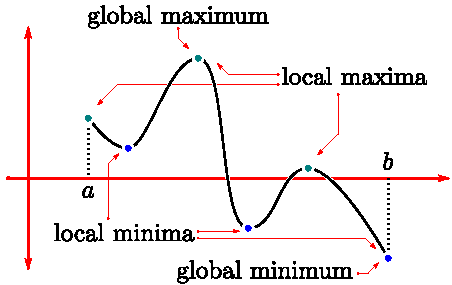
\includegraphics[scale=0.9,page=1]{fig/maxmin3.pdf}
  \hspace{25mm}
  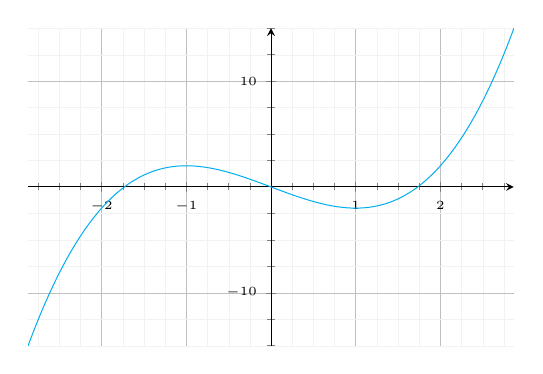
\begin{tikzpicture}[scale=0.9]
    \begin{axis}%
      [grid=both,
       unit vector ratio={8 1},
       minor tick num=3,
       ymin=-15,ymax=15,
       grid style={line width=.1pt, draw=gray!10},
       major grid style={line width=.2pt,draw=gray!50},
       axis lines=middle
      ]
      \addplot[domain=-3:3,samples=3000,smooth,cyan] {x^3 - 3 * x};
    \end{axis}
  \end{tikzpicture}
\end{figure}

\begin{ex}
  \begin{itemize}\setlength\itemsep{0em}
    \item[]
    \item $\ds f(x) = \frac{1}{x}$ 在 $I = \mathbb{R}$ 沒有最大值, 最小值. 
    \item $\ds f(x) = x$ 在 $I = (0, 1)$ 沒有最大值, 最小值. 
    \item $\ds f(x) = x$ 在 $I = [0, 1]$ 有最大值 $1$, 最小值 $0$. 
    \item 若 $I = [-3,\,3]$, $\ds f(x) = x^3 - 3x$ 在 $x = 3$ 有最大值 $18$, 在 $x = -3$ 有最小值 $-18$, 在 $x = -1$ 有極大值 $2$, 在 $x = 1$ 有極小值 $-2$. 
  \end{itemize}
\end{ex}

%\begin{thm}
%  若函數在定義域為{\color{M4}有限閉區間}, 或{\color{M4}有限閉區間的有限聯集}連續, 則函數在定義域上有最大值及最小值. 
%\end{thm}
%
%\begin{thm}
%  若 $f(x)$ 在 $(a, b)$ 連續, 且 $\ds\lim_{x\to a+}f(x) = L$, $\ds\lim_{x\to b-}f(x) = M$. 
%  \begin{enumerate}\setlength\itemsep{0em}
%    \item 若 $\exists\,u\in(a, b)$ 使 $f(u) > L$ 且 $f(u) > M$, 則 $f$ 在 $(a, b)$ 有最大值. 
%    \item 若 $\exists\,u\in(a, b)$ 使 $f(u) < L$ 且 $f(u) < M$, 則 $f$ 在 $(a, b)$ 有最小值. 
%  \end{enumerate}
%  $a$ 可為 $-\infty$, $b$ 可為 $\infty$, $L$, $M$ 可為 $\pm\infty$. 
%\end{thm}

\begin{thm}
  若 $f$ 在 $c\in\dom f$ 有極值, 且 $f'(c)$ 存在, 則 $f'(c) = 0$. 
\end{thm}

\begin{fact}
  設 $f:I\to\mathbb{R}$ 在 $x_0\in I$ 有極值, 則 $x_0$ 為以下三情形之一: 
  %\setlength{\columnsep}{20mm}
  %\begin{multicols}{2}
    \begin{itemize}\setlength\itemsep{0em}
      \item 臨界點 (critical point) : $\ds f'(x_0) = 0$. 
      \item 奇異點 (singular point) : $f$ 在 $x_0$ 不可微.  
      \item $I$ 的邊界點 (boundary). 
    \end{itemize}
  %\end{multicols}
\end{fact}

\begin{ex}
  求 $f(x) = x^3 - 3 x^2 - 9x + 2$ 在 $[-2,\,2]$ 的最大值與最小值. 
\end{ex}

\begin{sol}
  \begin{itemize}\setlength\itemsep{0em}
    \item[]
    \item $f$ 在有限閉區間 $[-2,\,2]$ 連續, 故在 $[-2,\,2]$ 有最大值, 最小值. 
    \item 
      \begin{itemize}\setlength\itemsep{0em}
        \item $\ds f'(x) = 3 x^2 - 6 x - 9 = 3(x + 1)(x - 3)$, 在 $[-2,\,2]$ 之臨界點為 $-1$: $f(-1) = 7$. 
        \item $f$ 在 $[-2,\,2]$ 可微, 故無奇異點. 
        \item $[-2,\,2]$ 的邊界點為 $-2$ 與 $2$; $f(-2) = 0$, $f(2) = -20$. 
      \end{itemize}
      故最大值: $f(-1) = 7$, 最小值: $f(2) = -20$. 
  \end{itemize}
\end{sol}

%\begin{ex}
%  證明 $\ds f(x) = x + \frac{4}{x}$ 在 $\ds (0, \infty)$ 有最小值, 並求其值. 
%\end{ex}
%
%\begin{sol}
%  \begin{itemize}\setlength\itemsep{0em}
%    \item[]
%    \item 由 $\ds\lim_{x\to 0+}f(x) = \infty$, $\ds\lim_{x\to\infty}f(x) = \infty$, $f(1) = 5 < \infty$, $f$ 在 $(0, \infty)$ 有最小值. 
%    \item 
%      \begin{itemize}\setlength\itemsep{0em}
%        \item $\ds f'(x) = 1 - \frac{4}{x^2} = \frac{(x + 2)(x - 2)}{x^2}$, 臨界點為 $2$: $f(2) = 4$. 
%        \item $f$ 在 $(0, \infty)$ 可微, 無奇異點. 
%        \item $(0, \infty)$ 無邊界點. 
%      \end{itemize}
%      故 $f$ 在 $(0, \infty)$ 之最小值為 $f(2) = 4$. 
%  \end{itemize}
%\end{sol}
%
%\begin{ex}
%  求點 $(2,\,0)$ 到 $y^2 = x^2 + 1$ 之最短距離. 
%  \begin{center}
%    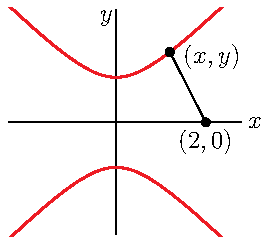
\includegraphics[scale=1]{fig/hyperbolaMaxMin.pdf}
%  \end{center}
%\end{ex}
%
%\begin{sol}
%  \begin{itemize}\setlength\itemsep{0em}
%    \item[]
%    \item 最小化距離平方 $\equiv$ 最小化距離. 
%    \item 令 $\ell$ 為 $(2, 0)$ 至 $y^2 = x^2 + 1$ 之距離: $\ds\ell^2 = (x - 2)^2 + y^2 = (x - 2)^2 + (x^2 + 1)$. 
%    \item 由 $\ds\ell^2(\pm\infty)=\infty$, $\ds\ell^2(0) = 5 < \infty$, $\ell^2$ 在 $(-\infty, \infty)$ 有最小值. 
%    \item 
%      \begin{itemize}\setlength\itemsep{0em}
%        \item $\ds\diff{}{x} \ell^2(x) = 2(x - 2) + 2x = 4(x - 1)$, 臨界點為 $1$; $\ell^2(1) = (1 - 2)^2 + (1 + 1) = 3\ie \ell(1) = \sqrt{3}$. 
%        \item $\ell^2$ 在 $(-\infty,\,\infty)$ 可微, 無奇異點. 
%        \item $(-\infty,\,\infty)$ 無邊界點. 
%      \end{itemize}
%      故最短距離為 $\ell(1) = \sqrt{3}$. 
%    \end{itemize}
%\end{sol}

\section*{Taylor 展開式}

\begin{dfn}
  \begin{itemize}\setlength{\itemsep}{0pt}
    \item[]
    \item 給定 $f\in C^\infty(a, b)$,$x_0\in(a, b)$,$\ds\sum_{n = 0}^\infty\frac{f^{(n)}(x_0)}{n!}(x - x_0)^n$ 稱為 $f(x)$ 在 $x = x_0$ 之 Tayler 級數 / 展開式;若 $x_0 = 0$ 稱為 $f(x)$ 之 MacLaurin 級數 / 展開式。
    \item 給定 $f\in C^N(a, b)$,$x_0\in(a, b)$, $0\leqslant n\leqslant N$,$\ds\sum_{k = 0}^n\frac{f^{(k)}(x_0)}{k!}(x - x_0)^n$ 稱為 $f(x)$ 在 $x = x_0$ 之 $n$ 階 Tayler 多項式;若 $x_0 = 0$ 稱為 $f(x)$ 之 $n$ 階 MacLaurin 多項式。
  \end{itemize}
\end{dfn}

\begin{ex} 常用 Maclaurin 級數。
  \begin{enumerate}\setlength{\itemsep}{-1pt}
    \item $\ds \frac{1}{1 - x} = 1 + x + x^2 + x^3 + x^4 + x^5 + x^6 + x^7 + \cdots = \sum_{n = 0}^\infty x^n$, $\forall\,|x| < 1$.
    \item $\ds e^x = 1 + x + \frac{x^2}{2!} + \frac{x^3}{3!} + \frac{x^4}{4!} + \frac{x^5}{5!} + \frac{x^6}{6!} + \frac{x^7}{7!} + \cdots = \sum_{n = 0}^\infty\frac{x^n}{n!}$, $\forall\,x\in\mathbb{R}$.
  \end{enumerate}
\end{ex}

\section*{不定積分}

\begin{dfn}[反導函數]
  給定 $\ds F(x)$, 若 $\ds\frac{\text{d}}{\text{d}x} F(x) = f(x)$, 則稱 $F(x)$ 為 $f(x)$ 的反導函數 (antiderivative) .  
\end{dfn}

\begin{prp}若 $\ds F(x)$, $\ds G(x)$ 分別為 $f(x)$, $g(x)$ 的反導函數, $c\in\mathbb{R}$. 則
  \begin{itemize}\setlength{\itemsep}{0pt}
    \item $\ds F(x) + c$ 為 $f(x)$ 的反導函數. 
    \item $\ds c\,F(x)$ 為 $c\,f(x)$ 的反導函數. 
    \item $\ds F(x) + G(x)$ 為 $f(x) + g(x)$ 的反導函數. 
  \end{itemize}
\end{prp}

\begin{fact}
  \begin{itemize}\setlength{\itemsep}{0pt}
    \item[]
    \item $\ds\frac{\text{d}}{\text{d}x} F(x) = f(x)\ie \text{d} F(x) = f(x)\cdot\text{d}x \ie F(x) = \int f(x)\cdot\text{d}x = \int f(x)\,\text{d}x$
    \item $F(x)$ 為 $f(x)$ 的反導函數 $\ifff$ $f(x)$ 的反導函數為 $F(x)$ $\ifff$ $F(x)$ 的導函數為 $f(x)$ $\ifff$ $F(x)$ (對 $x$) 的微分為 $f(x)$ $\ifff$ $f(x)$ (對 $x$) 的 (不定) 積分為 $F(x)$ 
    \item $f(x)$ 的反導函數 $\equiv$ $f(x)$ (對 $x$) 的 (不定) 積分
    \item 基礎積分集: 以下 $\ds\alpha\ne -1$, $a\ne 0$. 
      \begin{table}[!htbp]
        \centering
        \begin{tabular}{c|ccc}
          \toprule
          \addlinespace[2mm]
          $\ds f(x)$ & $\ds x^\alpha$ & $\ds\frac{1}{x}$ & $\ds e^{a x}$  \\
          \addlinespace[2mm]
          \midrule
          \addlinespace[2mm]
          $\ds \int f(x)\,\text{d}x$ & $\ds\frac{1}{\alpha + 1}\,x^{\alpha + 1}$ & $\ds\ln |x|$ & $\ds\frac{1}{a}\,e^{a x}$ \\
          \addlinespace[2mm]
          \bottomrule
        \end{tabular}
      \end{table}
    \item (Liouville) {\color{M4} $\ds e^{-x^2}$, $\ds\frac{e^x}{x}$, $\ds\frac{1}{\ln x}$, $\ds x^x$ 無 (初等函數形式之) 反導函數!}
  \end{itemize}
\end{fact}

\begin{ex}
  \setlength{\columnsep}{-7mm}
  \begin{multicols}{2}
    \begin{enumerate}\setlength{\itemsep}{0pt}
      \item $\ds\int\!\sqrt{x}\,\text{d}x = \frac{2}{3}\,x^{\frac{3}{2}} + c$
      \item $\ds\int x^\pi\,\text{d}x = \frac{1}{\pi + 1}\,x^{\pi + 1} + c$
      \item $\ds\int e^{-2x}\,\text{d}x = -\frac{1}{2}\,e^{-2 x} + c$
      \item $\ds\int\!\big(\frac{\pi}{x} - e^{\pi x}\big)\,\text{d}u = \pi\ln x - \frac{e^{\pi x}}{\pi} + c$
    \end{enumerate} 
  \end{multicols}
\end{ex}

\begin{exe} 求下列不定積分. 
  \setlength{\columnsep}{-2cm}
  \begin{multicols}{2}
    \begin{enumerate}\setlength{\itemsep}{0pt}
      \item $\ds\int\!\frac{x^3 - 1}{x^3}\,\mathrm{d}x {\color{C2}\;= x + \frac{1}{2x^3} + c}$
      \item $\ds\int\!5 - \frac{1}{\sqrt{x}}\,\mathrm{d}x {\color{C2}\;= 5x - 2\sqrt{x} + c}$
      \item $\ds\int\!(t - 1)(t + 1)\,\mathrm{d}t {\color{C2}\;= \frac{t^3}{3} - t + c}$
      \item $\ds\int\!(\sqrt{x} + 1)^2\,\mathrm{d}x {\color{C2}\;= \frac{x^2}{2} + x + \frac{4 x^{\frac{3}{2}}}{3} + c}$
      \item $\ds\int\!x\sqrt{3x}\,\mathrm{d}x {\color{C2}\;= \frac{2\sqrt{3}}{5}\,x^{\frac{5}{2}} + c}$
      \item $\ds\int\!\frac{1}{x^3} - \frac{1}{x^5}\,\mathrm{d}x {\color{C2}\;= \frac{-1}{2x^2} + \frac{1}{4x^4} + c}$
    \end{enumerate} 
  \end{multicols}
\end{exe}
\subsection*{變數變換法}

\begin{fact}
  $\ds\frac{\text{d}}{\text{d}x}f(g(x)) = f'(g(x))\cdot g'(x) \ie \text{d}f(g(x)) = f'(g(x))\cdot g'(x)\,\text{d}x \ie f(g(x)) = \int f'(g(x))\cdot g'(x)\,\text{d}x$. 令 $\ds u = g(x)$, 則 $\ds\frac{\text{d}}{\text{d}x} u = g'(x)\ie \text{d} u = g'(x)\,\text{d}x$; 故 $\ds\int f'(g(x))\cdot g'(x)\,\text{d}x = \int f'(u)\,\text{d}u = f(u) + c = f(g(x)) + c$.  
\end{fact}

\begin{ex}
  求 $\ds\int\!\frac{x}{\sqrt{x + 1}}\,\mathrm{d}x$. 
\end{ex}

\begin{sol}
  \begin{itemize}
    \item[]
    \item (解一) 令 $\ds u = x + 1$, 則 $\ds x = u - 1$, $\ds\mathrm{d}u = \mathrm{d}x$. 故 $\ds\int\!\frac{x}{\sqrt{x + 1}}\,\mathrm{d}x = \int\!\frac{u - 1}{\sqrt{u}}\,\mathrm{d}u = \int\!u^{\frac{1}{2}} - u^{-\frac{1}{2}}\,\mathrm{d}u = \frac{2}{3}\,u^{\frac{3}{2}} - 2\sqrt{u} + c = \frac{2}{3}\,(x + 1)^{\frac{3}{2}} - 2\sqrt{x + 1} + c$. 
    \item (解二) $\ds\int\!\frac{x}{\sqrt{x + 1}}\,\mathrm{d}x = \int\!\frac{x + 1 - 1}{\sqrt{x + 1}}\,\mathrm{d}x = \int\!\sqrt{x + 1} - \frac{1}{\sqrt{x + 1}}\,\mathrm{d}x$. 令 $\ds u = x + 1$, 則 $\ds\mathrm{d}u = \mathrm{d}x$. 故 $\ds\int\!\sqrt{x + 1} - \frac{1}{\sqrt{x + 1}}\,\mathrm{d}x = \int\!u^{\frac{1}{2}} - u^{-\frac{1}{2}}\,\mathrm{d}u = \frac{2}{3}\,u^{\frac{3}{2}} - 2\sqrt{u} + c = \frac{2}{3}\,(x + 1)^{\frac{3}{2}} - 2\sqrt{x + 1} + c$. 
    \item (解三) 令 $\ds u = \sqrt{x + 1}$, 則 $\ds x = u^2 - 1$, $\ds\mathrm{d}u = \frac{1}{2\sqrt{x + 1}}\,\mathrm{d}x$ $\ie$ $\ds\frac{1}{\sqrt{x + 1}}\,\mathrm{d}x = 2\,\mathrm{d}u$. 故 $\ds\int\!\frac{x}{\sqrt{x + 1}}\,\mathrm{d}x = \int\!x\cdot\frac{1}{\sqrt{x + 1}}\,\mathrm{d}x = \int\!(u^2 - 1)\cdot2\,\mathrm{d}u = \frac{2}{3}\,u^3 - 2u + c = \frac{2}{3}\,(x + 1)^{\frac{3}{2}} - 2\sqrt{x + 1} + c$. 
  \end{itemize}
\end{sol}

\begin{ex}
  求 $\ds\int\!\frac{x}{x^2+1}\,\mathrm{d}x$. 
\end{ex}

\begin{sol}
  令 $\ds u = x^2 + 1$, 則 $\ds\mathrm{d}u = 2\,x\,\mathrm{d}x$ $\ie$ $\ds x\,\mathrm{d}x=\frac{1}{2}\,\mathrm{d}u$. 故 $\ds\int\!\frac{x}{x^2+1}\,\mathrm{d}x = \int\!\frac{1}{x^2+1}\cdot x\,\mathrm{d}x = \int\!\frac{1}{u}\cdot\frac{1}{2}\,\mathrm{d}u = \frac{1}{2}\ln|u| + c = \frac{1}{2}\ln(x^2 + 1) + c$. 
\end{sol}
    
\begin{ex}
  求 $\ds\int e^x\sqrt{1 + e^x}\,\mathrm{d}x$. 
\end{ex}

\begin{sol}
  令 $u = 1 + e^x$, 則 $\ds\mathrm{d}u = e^x\,\mathrm{d}x$. 故 $\ds\int e^x\sqrt{1 + e^x}\,\mathrm{d}x = \int \sqrt{1 + e^x}\cdot e^x\,\mathrm{d}x = \int\!\sqrt{u}\cdot\mathrm{d}u = \frac{u^{\frac{3}{2}}}{\frac{3}{2}} + c = \frac{2}{3}(1 + e^x)^{\frac{3}{2}} + c$
\end{sol}

\begin{exe} 以變數變換法求下列不定積分. 
  \setlength{\columnsep}{-2cm}
  \begin{multicols}{2}
    \begin{enumerate}\setlength{\itemsep}{0pt}
      \item $\ds\int\!\frac{1}{\sqrt{2 x - 1}}\,\mathrm{d}x {\color{C2}\;= \sqrt{2x - 1} + c}$
      \item $\ds\int\!\sqrt{7x + 4}\,\mathrm{d}x {\color{C2}\;= \frac{2}{21}\,(7x + 4)^{\frac{3}{2}} + c}$
      \item $\ds\int\!e^{\pi x - 1}\,\mathrm{d}x {\color{C2}\;= \frac{e^{\pi x - 1}}{\pi} + c}$
      \item $\ds\int\!(x^2 - 2x + 1)^{\frac{1}{3}}\,\mathrm{d}x {\color{C2}\;= \frac{3}{5}\,(x - 1)^{\frac{5}{3}} + c}$
      \item $\ds\int\!\frac{x}{\sqrt{1 + 2x^2}}\,\mathrm{d}x {\color{C2}\;= \frac{\sqrt{1 + 2x^2}}{2} + c}$
      \item $\ds\int\!x^2\sqrt{1 - x}\,\mathrm{d}x {\color{C2}\;= -\frac{2\,(1 - x)^{\frac{3}{2}}}{3} + \frac{4\,(1 - x)^{\frac{5}{2}}}{5} - \frac{2\,(1 - x)^{\frac{7}{2}}}{7}}$
    \end{enumerate} 
  \end{multicols}
\end{exe}

\begin{sol}
  \begin{enumerate}\setlength{\itemsep}{0pt}
    \item[]
    \item 令 $u = 2x - 1$, 則 $\ds\text{d}u = 2\,\text{d}x\ie \text{d}x = \frac{1}{2}\,\text{d}u$. 故 $\ds\int\!\frac{1}{\sqrt{2 x - 1}}\,\mathrm{d}x = \int\!\frac{1}{\sqrt{u}}\cdot\frac{1}{2}\,\text{d}u = \sqrt{u} + c = \sqrt{2 x - 1} + c$. 
    \item 令 $u = 7x + 4$, 則 $\ds\text{d}u = 7\,\text{d}x\ie \text{d}x = \frac{1}{7}\,\text{d}u$. 故 $\ds\int\!\sqrt{7 x + 4}\,\mathrm{d}x = \int\!\sqrt{u}\cdot\frac{1}{7}\,\text{d}u = \frac{1}{7}\cdot\frac{2}{3}\,u^{\frac{3}{2}} + c = \frac{2}{21}\,(7 x + 4)^{\frac{3}{2}} + c$. 
    \item 令 $u = \pi x - 1$, 則 $\ds\text{d}u = \pi\,\text{d}x\ie \text{d}x = \frac{1}{\pi}\,\text{d}u$. 故 $\ds\int\!e^{\pi x - 1}\,\mathrm{d}x = \int\!e^u\cdot\frac{1}{\pi}\,\text{d}u = \frac{1}{\pi}\,e^{u} + c = \frac{e^{\pi x - 1}}{\pi} + c$. 
    \item 令 $\ds u = x - 1$, 則 $\ds\text{d}u = \text{d}x$. 故 $\ds\int\!(x^2 - 2x + 1)^{\frac{1}{3}}\,\mathrm{d}x = \int\!(x - 1)^\frac{2}{3}\,\text{d}x = \int\!u^\frac{2}{3}\,\text{d}u = \frac{3}{5}\,u^\frac{5}{3} + c = \frac{3}{5}\,(x - 1)^\frac{5}{3} + c$. 
    \item 令 $\ds u = 1 + 2x^2$, 則 $\ds\text{d}u = 4x\,\text{d}x\ie x\,\text{d}x = \frac{1}{4}\,\text{d}u$. 故 $\ds\int\!\frac{x}{\sqrt{1 + 2x^2}}\,\mathrm{d}x = \int\!\frac{1}{\sqrt{1 + 2x^2}}\cdot x\,\mathrm{d}x = \int\!\frac{1}{\sqrt{u}}\cdot\frac{1}{4}\,\text{d}u = \frac{1}{4}\cdot 2\,u^\frac{1}{2} + c = \frac{\sqrt{1 + 2x^2}}{2} + c$. 
    \item 令 $\ds u = \sqrt{1 - x}$, 則 $\ds u^2 = 1 - x\ie x = 1 - u^2$, $\text{d}x = -2\,u\,\text{d}u$. 故 $\ds\int\!x^2\sqrt{1 - x}\,\mathrm{d}x = \int\!(1 - u^2)^2\cdot u\cdot(-2)\,u\,\mathrm{d}u = -2\int\!(1 - u^2)^2\cdot u^2\,\text{d}u = -2\int\!\big(u^2 - 2u^4 + u^6\big)\,\text{d}u = -\frac{2\,u^3}{3} + \frac{4\,u^5}{5} - \frac{2\,u^7}{7} + c = -\frac{2\,(1 - x)^{\frac{3}{2}}}{3} + \frac{4\,(1 - x)^{\frac{5}{2}}}{5} - \frac{2\,(1 - x)^{\frac{7}{2}}}{7}$. 
  \end{enumerate}
\end{sol}

\begin{exe} 以變數變換法求下列不定積分. 
  \setlength{\columnsep}{-1cm}
  \begin{multicols}{2}
    \begin{enumerate}\setlength{\itemsep}{0pt}
      \item $\ds\int\!x e^{-\frac{x^2}{2}}\,\mathrm{d}x {\color{C2}\;= -e^{-\frac{x^2}{2}} + c}$
      \item $\ds\int\!x^2 2^{x^3 + 1}\,\mathrm{d}x {\color{C2}\;= \frac{2^{x^3 + 1}}{3\ln 2} + c}$
      \item $\ds\int\!\frac{\ln x}{x}\,\mathrm{d}x {\color{C2}\;= \frac{1}{2}\,(\ln x)^2 + c}$
      \item $\ds\int\!\frac{x + 1}{\sqrt{x^2 + 2x + 3}}\,\mathrm{d}x {\color{C2}\;= \sqrt{x^2 + 2x + 3} + c}$
    \end{enumerate} 
  \end{multicols}
\end{exe}

\begin{sol}
  \begin{enumerate}\setlength{\itemsep}{0pt}
    \item[]
    \item 令 $\ds u = \frac{x^2}{2}$, 則 $\ds\text{d}u = x\,\text{d}x$, 故 $\ds\int x e^{-\frac{x^2}{2}}\,\mathrm{d}x = \int e^{-\frac{x^2}{2}}\cdot x\,\mathrm{d}x = \int e^{-u}\,\text{d}u = -e^{-u} + c = -e^{-\frac{x^2}{2}} + c$
    \item 令 $\ds u = x^3 + 1$, 則 $\ds\text{d} u = 3 x^2\,\text{d}x\ie x^2\,\text{d}x = \frac{1}{3}\,\text{d}u$, 故 $\ds\int x^2 2^{x^3 + 1}\,\mathrm{d}x = \int 2^{x^3 + 1}\cdot x^2\,\text{d}x = \int 2^u\cdot\frac{1}{3}\,\text{d}u = \frac{1}{3}\int e^{u\ln 2}\,\text{d}u = \frac{1}{3\ln 2}e^{u\ln 2} + c = \frac{2^{x^3 + 1}}{3\ln 2} + c$
    \item 令 $\ds u = \ln x$, 則 $\ds\text{d} u = \frac{1}{x}\,\text{d}x$, 故 $\ds\int\!\frac{\ln x}{x}\,\mathrm{d}x = \int\!\ln x\cdot\frac{1}{x}\,\text{d}x = \int u\,\text{d}u = \frac{1}{2} u^2 + c = \frac{1}{2}\,(\ln x)^2 + c$
    \item 令 $\ds u = x^2 + 2x + 3$, 則 $\ds\text{d} u = (2 x + 2)\,\text{d}x\ie (x + 1)\,\text{d}x = \frac{1}{2}\,\text{d}u$, 故 $\ds\int\!\frac{x + 1}{\sqrt{x^2 + 2x + 3}}\,\mathrm{d}x = \int\!\frac{1}{\sqrt{x^2 + 2x + 3}}\cdot(x + 1)\,\text{d}x = \int\!\frac{1}{\sqrt{u}}\cdot\frac{1}{2}\,\text{d}u = \sqrt{u} + c = \sqrt{x^2 + 2x + 3} + c$
  \end{enumerate}
\end{sol}

\subsection*{部份積分法}

\begin{fact}
  $\ds\frac{\mathrm{d}}{\mathrm{d}x}\,(u(x)\,v(x)) = u(x)\,\frac{\mathrm{d}v(x)}{\mathrm{d}x} + v(x)\,\frac{\mathrm{d}u(x)}{\mathrm{d}x}\ie u(x)\,v(x) = \int u(x)\,\mathrm{d}v(x) + \int v(x)\,\mathrm{d}u(x) \\ \ie \int u\,\text{d}v = u\,v - \int v\,\text{d}u$. 
\end{fact}

\begin{ex}
  求 $\ds\int x\, e^{x}\,\mathrm{d}x$. 
\end{ex}

\begin{sol}
  令 $u = x$, 則 $\ds\mathrm{d}u = \mathrm{d}x$. 令 $\ds\mathrm{d}v = e^x\,\mathrm{d}x$, 則 $\ds v = e^x$. 故 $\ds\int x\, e^{x}\,\mathrm{d}x = x\cdot e^x - \int e^x\,\mathrm{d}x = xe^x - e^x + c$. 
\end{sol}
    
\begin{ex}
  求 $\ds\int\!\ln x\,\mathrm{d}x$. 
\end{ex}

\begin{sol}
  令 $\ds u = \ln x$, 則 $\ds\mathrm{d}u = \frac{1}{x}\mathrm{d}x$. 令 $\ds\mathrm{d}v = \mathrm{d}x$, 則 $v = x$. 故 $\ds\int\!\ln x\,\mathrm{d}x = \ln x \cdot x - \int x\cdot\frac{1}{x}\,\mathrm{d}x = x\ln x - x + c$. 
\end{sol}

\subsection*{列表法}

\begin{fact}
  \begin{enumerate}\setlength{\itemsep}{0pt}
    \item[]
    \item 將要微分函數寫左邊, 積分函數寫右邊; 左邊連續微分, 右邊連續積分
    \item 依序左上連右下斜線函數相乘, 最底部水平兩邊函數相乘並積分, 符號正負相間
    \item 將上式所得項全部加總即為所求積分
  \end{enumerate}
\end{fact}

\begin{ex}
  求 $\ds\int (x + 3)\,e^{2x}\,\mathrm{d}x$. 
\end{ex}

\begin{sol} 
  \begin{minipage}{0.45\textwidth}
    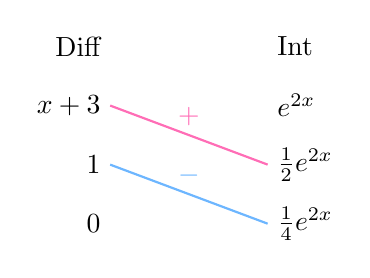
\begin{tikzpicture}[yscale=0.75]
      \draw (-1, 1) node[left]{Diff};
      \draw (1,  1) node[right]{Int};
      \draw (-1, -0) node[left]{$x+3$};
      \draw (1,  -0) node[right]{$e^{2x}$};
      \draw (-1, -1) node[left]{$1$};
      \draw (-1, -2) node[left]{$0$};
      \draw (1,  -1) node[right]{$\frac{1}{2}e^{2x}$};
      \draw (1,  -2) node[right]{$\frac{1}{4}e^{2x}$};
      \draw[thick, M4, -] (-1, -0)--(1, -1); \draw[M4] (0, -0.5) node[above]{$+$};
      \draw[thick, C4, -] (-1, -1)--(1, -2); \draw[C4] (0, -1.5) node[above]{$-$};
    \end{tikzpicture}
  \end{minipage}
  \hspace{5mm}
  \begin{minipage}{0.5\textwidth}
     $\ds\int (x + 3)\,e^{2x}\,\mathrm{d}x = (x + 3)\,\frac{1}{2}e^{2x} - \frac{1}{4}e^{2x}$
  \end{minipage}
\end{sol}

\begin{ex}
  求 $\ds\int (x^2 - 2x)\,e^{kx}\,\mathrm{d}x$. 
\end{ex}

\begin{sol} 
  \begin{minipage}{0.35\textwidth}
    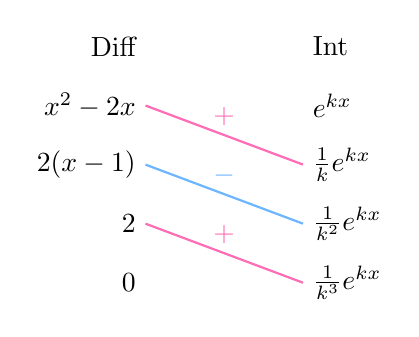
\begin{tikzpicture}[yscale=0.75]
      \draw (-1, 1) node[left]{Diff};
      \draw (1,  1) node[right]{Int};
      \draw (-1, -0) node[left]{$x^2 - 2x$};
      \draw (1,  -0) node[right]{$e^{kx}$};
      \draw (-1, -1) node[left]{$2(x - 1)$};
      \draw (-1, -2) node[left]{$2$};
      \draw (-1, -3) node[left]{$0$};
      \draw (1,  -1) node[right]{$\frac{1}{k}e^{kx}$};
      \draw (1,  -2) node[right]{$\frac{1}{k^2}e^{kx}$};
      \draw (1,  -3) node[right]{$\frac{1}{k^3}e^{kx}$};
      \draw[thick, M4, -] (-1, -0)--(1, -1); \draw[M4] (0, -0.5) node[above]{$+$};
      \draw[thick, C4, -] (-1, -1)--(1, -2); \draw[C4] (0, -1.5) node[above]{$-$};
      \draw[thick, M4, -] (-1, -2)--(1, -3); \draw[M4] (0, -2.5) node[above]{$+$};
    \end{tikzpicture}
  \end{minipage}
  \hspace{5mm}
  \begin{minipage}{0.6\textwidth}
    $\ds\int (x^2 - 2x)\,e^{kx}\,\mathrm{d}x = (x^2 - 2x)\,\frac{1}{k}e^{kx} - 2(x-1)\frac{1}{k^2}e^{kx} + 2\frac{1}{k^3}e^{kx}$
  \end{minipage}
\end{sol}

\begin{ex}
  求 $\ds\int x^5\,e^{ax}\,\mathrm{d}x$. 
\end{ex}

\begin{sol} 
  \begin{minipage}{0.3\textwidth}
    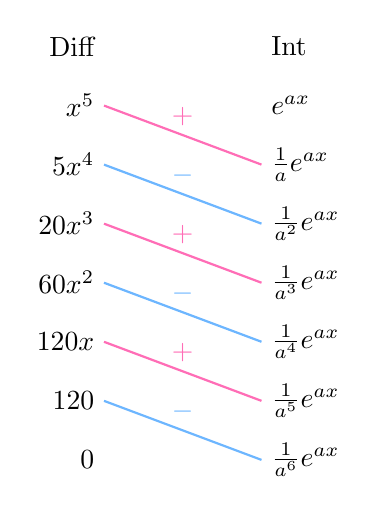
\begin{tikzpicture}[yscale=0.75]
      \draw (-1, 1) node[left]{Diff};
      \draw (1,  1) node[right]{Int};
      \draw (-1, -0) node[left]{$x^5$};
      \draw (1,  -0) node[right]{$e^{ax}$};
      \draw (-1, -1) node[left]{$5x^4$};
      \draw (-1, -2) node[left]{$20x^3$};
      \draw (-1, -3) node[left]{$60x^2$};
      \draw (-1, -4) node[left]{$120x$};
      \draw (-1, -5) node[left]{$120$};
      \draw (-1, -6) node[left]{$0$};
      \draw (1,  -1) node[right]{$\frac{1}{a}e^{ax}$};
      \draw (1,  -2) node[right]{$\frac{1}{a^2}e^{ax}$};
      \draw (1,  -3) node[right]{$\frac{1}{a^3}e^{ax}$};
      \draw (1,  -4) node[right]{$\frac{1}{a^4}e^{ax}$};
      \draw (1,  -5) node[right]{$\frac{1}{a^5}e^{ax}$};
      \draw (1,  -6) node[right]{$\frac{1}{a^6}e^{ax}$};
      \draw[thick, M4, -] (-1, -0)--(1, -1); \draw[M4] (0, -0.5) node[above]{$+$};
      \draw[thick, C4, -] (-1, -1)--(1, -2); \draw[C4] (0, -1.5) node[above]{$-$};
      \draw[thick, M4, -] (-1, -2)--(1, -3); \draw[M4] (0, -2.5) node[above]{$+$};
      \draw[thick, C4, -] (-1, -3)--(1, -4); \draw[C4] (0, -3.5) node[above]{$-$};
      \draw[thick, M4, -] (-1, -4)--(1, -5); \draw[M4] (0, -4.5) node[above]{$+$};
      \draw[thick, C4, -] (-1, -5)--(1, -6); \draw[C4] (0, -5.5) node[above]{$-$};
    \end{tikzpicture}
  \end{minipage}
  \hspace{5mm}
  \begin{minipage}{0.65\textwidth}
    $\ds\int x^5\,e^{ax}\,\mathrm{d}x \\ = x^5\,\frac{1}{a}e^{ax} - 5x^4\,\frac{1}{a^2}e^{ax} + 20x^3\,\frac{1}{a^3}e^{ax} - 60x^2\,\frac{1}{a^4}e^{ax} + 120x\,\frac{1}{a^5}e^{ax} - 120\,\frac{1}{a^6}e^{ax} \\ = \bigg(\frac{x^5}{a}-\frac{5x^4}{a^2} + \frac{20x^3}{a^3} - \frac{60x^2}{a^4} + \frac{120x}{a^5} - \frac{120}{a^6}\bigg)\,e^{ax}$
  \end{minipage}
\end{sol}

\begin{exe} 以部份積分法求下列不定積分. 注意: 可能會因為常數項而跟此處答案不同. 
  \begin{enumerate}\setlength{\itemsep}{0pt}
    \item $\ds\int x^3\ln x\,\mathrm{d}x {\color{C2}\;= \frac{x^4}{4}\ln x -\frac{x^4}{16} + c}$
    \item $\ds\int x(\ln x)^3\,\mathrm{d}x {\color{C2}\;= \frac{x^2}{2}\Big((\ln x)^3 -\frac{3(\ln x)^2}{2} + \frac{3\ln x}{2} - \frac{3}{4} \Big) + c}$
    \item $\ds\int x^5 e^{-x^2}\,\mathrm{d}x {\color{C2}\;= -\frac{1}{2}e^{-x^2}(x^4 + 2x^2 + 2) + c}$
    \item $\ds\int x e^{\sqrt{x}}\,\mathrm{d}x {\color{C2}\;= 2\,e^{\sqrt{x}}\,\big(x\sqrt{x} - 3x + 6\sqrt{x} - 6\big) + c}$
    \item $\ds\int\!\frac{x e^x}{(x + 1)^2}\,\mathrm{d}x {\color{C2}\;= \frac{e^x}{x + 1} + c}  $
   % \item $\ds\int\!\frac{\ln x}{\sqrt{1 + x}}\,\mathrm{d}x {\color{C2}\;= \ln x\cdot 2\sqrt{1 + x} - 4\sqrt{1+x} - 2\ln(\sqrt{1 + x}-1) + 2\ln(\sqrt{1+x} + 1) + c}$
  \end{enumerate}
\end{exe}

\begin{sol}
  \begin{enumerate}\setlength{\itemsep}{0pt}
    \item[]
    \item 令 $\ds u = \ln x$, 則 $\ds\text{d}u = \frac{1}{x}\,\text{d}x$; $\ds\text{d}v = x^3\,\text{d}x$, 則 $\ds v = \frac{x^4}{4}$.  故 $\ds\int x^3\ln x\,\mathrm{d}x = \ln x\cdot\frac{x^4}{4} - \int\!\frac{x^4}{4}\cdot\frac{1}{x}\,\text{d}x = \ln x\cdot\frac{x^4}{4} - \int\!\frac{x^3}{4}\,\text{d}x = \ln x\cdot\frac{x^4}{4} - \frac{x^4}{16} + c$.   
    \item 令 $\ds u = (\ln x)^3$, 則 $\ds\text{d}u = 3(\ln x)^2\cdot\frac{1}{x}\,\text{d}x$; $\ds\text{d}v = x\,\text{d}x$, 則 $\ds v = \frac{x^2}{2}$.  故 $\ds\int x(\ln x)^3\,\mathrm{d}x = (\ln x)^3\cdot\frac{x^2}{2} - \int\!\frac{x^2}{2}\cdot 3(\ln x)^2\cdot\frac{1}{x}\,\text{d}x = (\ln x)^3\cdot\frac{x^2}{2} - \frac{3}{2}\int x(\ln x)^2\,\text{d}x$. 令 $\ds u = (\ln x)^2$, 則 $\ds\text{d}u = 2\,\ln x\cdot\frac{1}{x}\,\text{d}x$; $\ds\text{d}v = x\,\text{d}x$, 則 $\ds v = \frac{x^2}{2}$.  故 $\ds\int x(\ln x)^2\,\text{d}x = (\ln x)^2\cdot\frac{x^2}{2} - \int\!\frac{x^2}{2}\cdot 2\ln x\cdot\frac{1}{x}\,\text{d}x = (\ln x)^2\cdot\frac{x^2}{2} - \int x\ln x\,\text{d}x$. 令 $\ds u = \ln x$, 則 $\ds\text{d}u = \frac{1}{x}\,\text{d}x$; $\ds\text{d}v = x\,\text{d}x$, 則 $\ds v = \frac{x^2}{2}$. 故 $\ds\int x\ln x\,\text{d}x = \ln x\cdot\frac{x^2}{2} - \int\!\frac{x^2}{2}\cdot\frac{1}{x}\,\text{d}x = \ln x\cdot\frac{x^2}{2} - \frac{1}{2}\int x\,\text{d}x = \ln x\cdot\frac{x^2}{2} - \frac{x^2}{4}$. 以上, $\ds\int x(\ln x)^3\,\mathrm{d}x = (\ln x)^3\cdot\frac{x^2}{2} - \frac{3}{2}\Big((\ln x)^2\cdot\frac{x^2}{2} - \big(\ln x\cdot\frac{x^2}{2} - \frac{x^2}{4}\big)\Big) = \frac{x^2}{2}\big((\ln x)^3 - \frac{3(\ln x)^2}{2} + \frac{3\ln x}{2} - \frac{3}{4}\big) + c$
    \item 令 $\ds w = x^2$, 則 $\ds\text{d}w = 2x\,\text{d}x\ie x\,\text{d}x = \frac{1}{2}\,\text{d}w$, 故 $\ds\int x^5 e^{-x^2}\,\text{d}x = \int e^{-x^2}\cdot(x^2)^2\cdot x\,\text{d}x = \int e^{-w}\cdot w^2\cdot\frac{1}{2}\,\text{d}w = \frac{1}{2}\int w^2\,e^{-w}\,\text{d}w = -\frac{1}{2}\,e^{-w}(w^2 + 2w + 2) = -\frac{1}{2}\,e^{-x^2}(x^4 + 2x^2 + 2) + c$. \\
  \begin{minipage}{0.15\textwidth}
    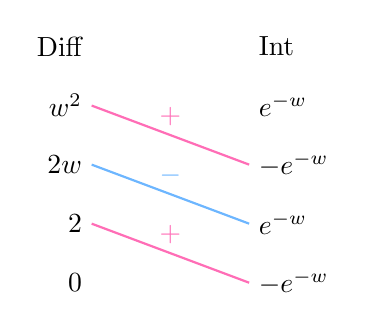
\begin{tikzpicture}[yscale=0.75]
      \draw (-1, 1) node[left]{Diff};
      \draw (1,  1) node[right]{Int};
      \draw (-1, -0) node[left]{$w^2$};
      \draw (1,  -0) node[right]{$e^{-w}$};
      \draw (-1, -1) node[left]{$2w$};
      \draw (-1, -2) node[left]{$2$};
      \draw (-1, -3) node[left]{$0$};
      \draw (1,  -1) node[right]{$-e^{-w}$};
      \draw (1,  -2) node[right]{$e^{-w}$};
      \draw (1,  -3) node[right]{$-e^{-w}$};
      \draw[thick, M4, -] (-1, -0)--(1, -1); \draw[M4] (0, -0.5) node[above]{$+$};
      \draw[thick, C4, -] (-1, -1)--(1, -2); \draw[C4] (0, -1.5) node[above]{$-$};
      \draw[thick, M4, -] (-1, -2)--(1, -3); \draw[M4] (0, -2.5) node[above]{$+$};
    \end{tikzpicture}
  \end{minipage}
  \hspace{5mm}
  \begin{minipage}{0.8\textwidth}
    \begin{align*}
      \int w^2 e^{-w}\,\mathrm{d}w = -w^2\,e^{-w} - 2w\,e^{-w} - 2\,e^{-w} = -e^{-w}(w^2 + 2w + 2)
    \end{align*}
  \end{minipage}
\item 令 $\ds w = \sqrt{x}$, 則 $\ds w^2 = x$, $\ds\text{d}x = 2w\,\text{d}w$, 故 $\ds\int x e^{\sqrt{x}}\,\mathrm{d}x = \int w^2 e^w\cdot 2w\,\text{d}w = 2\int w^3 e^w\,\text{d}w = 2\,e^w(w^3 - 3w^2 + 6w - 6) = 2\,e^{\sqrt{x}}\,(x\sqrt{x} - 3 x + 6\sqrt{x} - 6) + c$ \\ 
  \begin{minipage}{0.15\textwidth}
    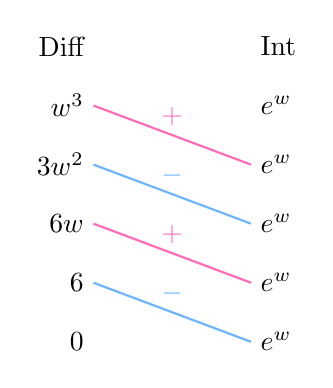
\begin{tikzpicture}[yscale=0.75]
      \draw (-1, 1) node[left]{Diff};
      \draw (1,  1) node[right]{Int};
      \draw (-1, -0) node[left]{$w^3$};
      \draw (1,  -0) node[right]{$e^w$};
      \draw (-1, -1) node[left]{$3w^2$};
      \draw (-1, -2) node[left]{$6w$};
      \draw (-1, -3) node[left]{$6$};
      \draw (-1, -4) node[left]{$0$};
      \draw (1,  -1) node[right]{$e^w$};
      \draw (1,  -2) node[right]{$e^w$};
      \draw (1,  -3) node[right]{$e^w$};
      \draw (1,  -4) node[right]{$e^w$};
      \draw[thick, M4, -] (-1, -0)--(1, -1); \draw[M4] (0, -0.5) node[above]{$+$};
      \draw[thick, C4, -] (-1, -1)--(1, -2); \draw[C4] (0, -1.5) node[above]{$-$};
      \draw[thick, M4, -] (-1, -2)--(1, -3); \draw[M4] (0, -2.5) node[above]{$+$};
      \draw[thick, C4, -] (-1, -3)--(1, -4); \draw[C4] (0, -3.5) node[above]{$-$};
    \end{tikzpicture}
  \end{minipage}
  \hspace{5mm}
  \begin{minipage}{0.8\textwidth}
    \begin{align*}
      \int w^3\,e^w\,\mathrm{d}w = w^3\,e^w - 3w^2\,e^w + 6w\,e^w - 6\,e^w = e^w(w^3 - 3w^2 + 6w - 6)
    \end{align*}
  \end{minipage}
    \item $\ds\int\!\frac{x e^x}{(x + 1)^2}\,\text{d}x = \int\!\frac{(x + 1 - 1)e^x}{(x + 1)^2}\,\text{d}x = \int\!\frac{e^x}{x + 1}\,\text{d}x - \int\!\frac{e^x}{(x + 1)^2}\,\text{d}x$. 令 $\ds u = e^x$, 則 $\ds\text{d}u = e^x\,\text{d}x$; $\ds\text{d}v = \frac{1}{(x + 1)^2}\,\text{d}x$, 則 $\ds v = \frac{-1}{x + 1}$. 故 $\ds\int\!\frac{e^x}{(x + 1)^2}\,\mathrm{d}x = e^x\cdot\frac{-1}{x + 1} + \int\!\frac{1}{x + 1}\cdot e^x\,\text{d}x = \frac{-e^x}{x + 1} + \int\!\frac{e^x}{x + 1}\,\text{d}x$; 原式 $\ds\int\!\frac{x e^x}{(x + 1)^2}\,\text{d}x = \int\!\frac{e^x}{x + 1}\,\text{d}x - \int\!\frac{e^x}{(x + 1)^2}\,\text{d}x = \int\!\frac{e^x}{x + 1}\,\text{d}x - \Big(\frac{-e^x}{x + 1} + \int\!\frac{e^x}{x + 1}\,\text{d}x\Big) = \frac{e^x}{x + 1}$. 
 % \item 令 $\ds u = \ln x$, 則 $\ds\text{d}u = \frac{1}{x}\,\text{d}x$; $\ds\text{d}v = \frac{1}{\sqrt{1 + x}}\,\text{d}x$, 則 $\ds v = 2\sqrt{1 + x}$. 故 $\ds\int\!\frac{\ln x}{\sqrt{1 + x}}\,\text{d}x = \ln x\cdot 2\sqrt{1 + x} - 2 \int\!\frac{\sqrt{1 + x}}{x}\,\text{d}x$. 令 $\ds w = \sqrt{1 + x}$, 則 $\ds w^2 = 1 + x \ie x= w^2 - 1$, $\ds 2w\,\text{d}w = \text{d}x$, 故 $\ds\int\!\frac{\sqrt{1 + x}}{x}\,\text{d}x = \int\!\frac{w}{w^2 - 1}\cdot 2w\,\text{d}w = 2\int\!\frac{w^2}{w^2 - 1}\,\text{d}w = 2\int\!\frac{(w^2 - 1) + 1}{w^2 - 1}\,\text{d}w = 2 w + 2\int\!\frac{1}{w^2 - 1}\,\text{d}w = 2\sqrt{1 + x} + 2\int\!\frac{1}{w^2 -1}\,\text{d}w$. 由 $\ds\frac{1}{w^2 - 1} = \frac{1}{2}\,\bigg(\frac{1}{w - 1} - \frac{1}{w + 1}\bigg)$, $\ds\int\!\frac{1}{w^2 - 1}\,\text{d}w = \frac{1}{2}\int\!\Big(\frac{1}{w - 1} - \frac{1}{w + 1}\Big)\,\text{d}w =\frac{1}{2}\,\big(\ln|w - 1| - \ln|w + 1|\big) = \frac{1}{2}\,\big(\ln|\sqrt{1 + x} - 1| - \ln|\sqrt{1 + x} + 1|\big)$. 以上, $\ds\int\!\frac{\ln x}{\sqrt{1 + x}}\,\mathrm{d}x = \ln x\cdot 2\sqrt{1 + x} - 2\,\big(2\sqrt{1+x} + 2\,\big(\frac{1}{2}\,\big(\ln|\sqrt{1 + x} - 1| - \ln|\sqrt{1 + x} + 1|\big)\big)\big) = \ln x\cdot 2\sqrt{1 + x} - 4\sqrt{1 + x} - 2\ln|\sqrt{1 + x} - 1| + 2\ln|\sqrt{1 + x} + 1| + c$. 
  \end{enumerate}
\end{sol}

\section*{定積分}

定積分 $\approx$  (帶符號) 面積: $x$ 軸上方為正, 下方為負. 

\begin{dfn}
  給定 $f:[a,\,b]\to\mathbb{R}$. 
  \begin{itemize}\setlength{\itemsep}{0pt}
    \item $[a,\,b]$ 分割 $\ds\mathbb{P}: a = x_0 < x_1 < x_2 < \cdots < x_n = b$
    \item $\ds\Delta x_k=x_k - x_{k-1}$, $k=1,\,2,\,\ldots,\,n$; $\ds\|\mathbb{P}\| = \max\{\,|\Delta x_k|\;|\;1\leqslant k\leqslant n\}$
    \item 樣本點 $\ds\xi_k$: $\ds x_{k-1} \leqslant \xi_k \leqslant x_k$, $k=1,\,2,\,\ldots,\,n$
    \item $\ds u_k = \sup\left\{\,f(x)\;|\;x_{k-1}\leqslant x\leqslant x_k\right\}$, $l_k = \inf\left\{\,f(x)\;|\;x_{k-1}\leqslant x\leqslant x_k\right\}$, $k=1,\,2,\,\ldots,\,n$
    \item $\ds R(f,\mathbb{P}) = \sum_{k=1}^n f(\xi_k)\,\Delta x_k$, $\ds U(f,\mathbb{P}) = \sum_{k=1}^n u_k\,\Delta x_k$, $\ds L(f,\mathbb{P}) = \sum_{k=1}^n l_k\,\Delta x_k$; \\顯然 $\ds L(f,\mathbb{P})\leqslant R(f,\mathbb{P})\leqslant U(f, \mathbb{P})$. 
    \item 求 $\ds\lim_{\|\mathbb{P}\|\to 0} R(f,\mathbb{P})$. 若對不同分割與樣本點選取此極限均存在且相等, 稱 $f$ 在 $[a, b]$ 可積 (分) ; $f(x)$ 在 $[a,\,b]$ 的定積分 $\ds\int_a^b f(x)\,\mathrm{d}x \equiv \lim_{\|\mathbb{P}\|\to 0} R(f,\mathbb{P})$
  \end{itemize}
\end{dfn}

\begin{rmk}
  \begin{itemize}\setlength{\itemsep}{0pt}
    \item[]
    \item 在 $\ds\int_a^b f(x)\,\text{d}x$ 中, $a$ 為\emph{積分下限} (lower limit of integration) , $b$ 為\emph{積分上限} (upper limit of integration) , $f(x)$ 為\emph{被積分式} (integrand) , $x$ 為\emph{積分變數} (variable of integration) . 
    \item $\ds\int_a^b f(x)\,\text{d}x = \int_a^b f(t)\,\text{d}t = \int_a^b f(u)\,\text{d}u$  (定積分數值與積分變數無關) 
  \end{itemize}
\end{rmk}

\begin{fact}
  若 $f$ 在 $[a,\,b]$ 連續, 則 $f$ 在 $[a,\,b]$ 可積. 
\end{fact}

\begin{prp}
  令 $f$, $g$ 在包含 $a$, $b$, $c$ 之區間為可積, $\alpha$, $\beta\in\mathbb{R}$. 則
  \begin{multicols}{2}
    \begin{enumerate}\setlength{\itemsep}{0pt}
      \item $\ds\int_a^a f(x)\,\mathrm{d}x = 0$
      \item $\ds\int_a^b f(x)\,\mathrm{d}x = -\int_b^a f(x)\,\mathrm{d}x$
      \item $\ds\int_a^b \big(\alpha\,f(x) + \beta\,g(x)\big)\,\mathrm{d}x = \alpha\int_a^b f(x)\,\mathrm{d}x + \beta\int_a^b g(x)\,\mathrm{d}x$
      \item $\ds\int_a^b f(x)\,\mathrm{d}x + \int_b^c f(x)\,\mathrm{d}x = \int_a^c f(x)\,\mathrm{d}x$
      \item $\ds\int_a^b f(x)\,\mathrm{d}x\leqslant\int_a^b g(x)\,\mathrm{d}x$, 若 $f(x)\leqslant g(x)\;\forall\,x\in[a, b],\;a\leqslant b$
      \item $\ds\left|\,\int_a^b f(x)\,\mathrm{d}x\,\right|\leqslant \int_a^b \left|\,f(x)\,\right|\,\mathrm{d}x, \quad a\leqslant b$ 
      \item $f(x)$ 為奇函數: $\ds\int_{-a}^a f(x)\,\mathrm{d}x = 0$
      \item $f(x)$ 為偶函數: $\ds\int_{-a}^a f(x)\,\mathrm{d}x = 2\int_0^a f(x)\,\mathrm{d}x$
    \end{enumerate}
  \end{multicols}
\end{prp}

\begin{ex}
  \begin{enumerate}\setlength{\itemsep}{0pt}
    \item[]
    \item $\ds\int_{-\sqrt{2}}^{\sqrt{2}} \sqrt{2 - x^2}\,\mathrm{d}x = \pi$ (半徑 $\sqrt{2}$ 之半圓面積) 
    \item $\ds\int_{-4}^{4} \big(e^{x} - e^{-x}\big)\,\mathrm{d}x = 0$ ($e^{x} - e^{-x}$ 為奇函數) 
    \item $\ds\int_{-2024}^{2024} \big(e^{9x^5-2x^7} - e^{-9x^5 + 2x^7}\big)\,\mathrm{d}x = 0$ ($e^{9x^5-2x^7} - e^{-9x^5 + 2x^7}$ 為奇函數)  
    \item $\ds\int_{-a}^a |x|\,\mathrm{d}x = 2\int_0^a |x|\,\mathrm{d}x = a^2$ ($|x|$ 為偶函數; 兩 $a\times a$ 等腰直角三角形面積) 
    \item 定義 $\ds\int_1^x\frac{1}{\tau}\,\mathrm{d}\tau\equiv\ln x$, 則 $\ds\int_{\frac{1}{4}}^3\frac{1}{x}\,\mathrm{d}x = \int_{\frac{1}{4}}^1 \frac{1}{x}\,\mathrm{d}x + \int_1^3 \frac{1}{x}\,\mathrm{d}x = -\int_1^{\frac{1}{4}}\frac{1}{x}\,\mathrm{d}x + \int_1^3\frac{1}{x}\,\mathrm{d}x = \ln 12$
  \end{enumerate}
\end{ex}

\subsection*{微積分基本定理}

\begin{thm}[微積分基本定理 (Fundamental Theorem of Calculus, FTC) ]
  \begin{enumerate}\setlength{\itemsep}{0pt}
    \item[]
    \item 若 $f$ 在 $[a,\,b]$ 連續, 令 $\ds F(x) = \int_a^x f(\tau)\,\mathrm{d}\tau$ 且 $a\leqslant x\leqslant b$, 則 $\ds F'(x) = f(x)\;\forall\,x\in[a,\,b]$. 
    \item 若 $\ds G'(x) = f(x)\;\forall\,x\in[a,\,b]$, 則 $\ds\int_a^b f(x)\,\mathrm{d}x = G(b) - G(a) \equiv G(x)\,\Big|_a^b$. 
  \end{enumerate}
\end{thm}

\begin{rmk}
  由 FTC, $\ds\int_a^b f(x)\,\mathrm{d}x$ 可由 $f$ 的反導函數 (不定積分) 得出, 不需繁複極限計算!
\end{rmk}

\begin{ex}[以 FTC 求定積分]
  \begin{enumerate}\setlength{\itemsep}{0pt}
    \item[]
    \item $\ds x^2$ 之反導函數為 $\ds\frac{x^3}{3}$, 故 $\ds\int_0^1 x^2\,\text{d}x = \frac{1^3}{3} - \frac{0^3}{3} = \frac{1}{3}$. 
    \item $\ds e^x$ 之反導函數為 $\ds e^x$, 故 $\ds\int_0^1 e^x\,\text{d}x = e^1 - e^0 = e - 1$. 
  \end{enumerate}
\end{ex}

\begin{fact}[定積分變數變換]
  \begin{itemize}\setlength{\itemsep}{0pt}
    \item[]
    \item 求反導函數後代入: $\ds\int_a^b f'(g(x))\,g'(x)\,\text{d}x = f(g(x))\,\Big|_{x = a}^{x = b} = f(g(b)) - f(g(a))$
    \item 變數變換並改變積分範圍: $\ds\int_a^b f'(g(x))\,g'(x)\,\text{d}x = \int_a^b f'(g(x))\,\text{d}g(x) =\int_{g(a)}^{g(b)} f'(u)\,\text{d}u = f(u)\,\Big|_{u = g(a)}^{u = g(b)} = f(g(b)) - f(g(a))$
  \end{itemize}
\end{fact}

\begin{ex}
  求 $\ds\int_0^1 x^3(1 + x^4)^3\,\text{d}x$. 
\end{ex}

\begin{sol}
  \begin{itemize}\setlength{\itemsep}{0pt}
    \item[]
    \item 求反導函數後代入: 令 $\ds u = 1 + x^4$, 則 $\ds\text{d}u = 4 x^3\,\text{d}x\ie x^3\,\text{d}x = \frac{\text{d}u}{4}$, 故 $\ds\int x^3(1 + x^4)^3\,\text{d}x = \int (1 + x^4)^3\,x^3\,\text{d}x = \int u^3\,\frac{\text{d}u}{4} = \frac{u^4}{16} + c = \frac{(1 + x^4)^4}{16} + c$. 故 $\ds\int_0^1 x^3(1 + x^4)^3\,\text{d}x = \frac{(1 + x^4)^4}{16}\,\Big|_{x = 0}^{x = 1} = \frac{(1 + 1^4)^4 - (1 + 0^4)^4}{16} = \frac{15}{16}$. 
    \item 變數變換並改變積分範圍: 令 $\ds u = 1 + x^4$, 則 $\ds\text{d}u = 4 x^3\,\text{d}x\ie x^3\,\text{d}x = \frac{\text{d}u}{4}$. 積分範圍 $x$ 由 $0$ 至 $1$, 則變數變換後 $u$ 由 $\ds 1 + 0^4 = 1$ 至 $\ds1 + 1^4 = 2$, 故 $\ds\int_0^1 x^3(1 + x^4)^3\,\text{d}x = \int_0^1 (1 + x^4)^3\,x^3\,\text{d}x = \int_1^2 u^3\,\frac{\text{d}u}{4} = \frac{1}{4}\int_1^2 u^3\,\text{d}u = \frac{1}{16} u^4\,\Big|_{u = 1}^{u = 2} = \frac{2^4 - 1^4}{16} = \frac{15}{16}$. 
  \end{itemize}
\end{sol}

\begin{ex}
  求 $\ds\int_0^{\sqrt{3}}\frac{4x}{\sqrt{1 + x^2}}\,\text{d}x$. 
\end{ex}

\begin{sol}
  \begin{itemize}\setlength{\itemsep}{0pt}
    \item[]
    \item 求反導函數後代入: 令 $\ds u = 1 + x^2$, 則 $\ds\text{d}u = 2 x\,\text{d}x\ie 4x\,\text{d}x = 2\,\text{d}u$, 故 $\ds\int\!\frac{4x}{\sqrt{1 + x^2}}\,\text{d}x = \int\!\frac{2}{\sqrt{u}}\,\text{d}u = 4\sqrt{u} + c = 4\sqrt{1 + x^2} + c$. 故 $\ds\int_0^{\sqrt{3}}\frac{4x}{\sqrt{1 + x^2}}\,\text{d}x = 4\sqrt{1 + x^2}\,\Big|_{x = 0}^{x = \sqrt{3}} = 4\sqrt{1 + 3} - 4\sqrt{1} = 4$. 
    \item 變數變換並改變積分範圍: 令 $\ds u = 1 + x^2$, 則 $\ds\text{d}u = 2 x\,\text{d}x\ie 4x\,\text{d}x = 2\,\text{d}u$. 積分範圍 $x$ 由 $0$ 至 $\sqrt{3}$, 則變數變換後 $u$ 由 $\ds1 + 0^2 = 1$ 至 $\ds1 + (\sqrt{3})^2 = 4$, 故 $\ds\int_0^{\sqrt{3}}\frac{4x}{\sqrt{1 + x^2}}\,\text{d}x = \int_1^4 \frac{2}{\sqrt{u}}\,\text{d}u = 4\sqrt{u}\,\Big|_{u = 1}^{u = 4} = 4\,(\sqrt{4} - \sqrt{1}) = 4$. 
  \end{itemize}
\end{sol}

\begin{ex}
  若 $f$ 在 $[a, b]$ 二次可微且 $f(a) = f(b) = 0$, 證明 $\ds\int_a^b\!(x-a)(b-x)\,f''(x)\,\mathrm{d}x = -2\int_a^b\!f(x)\,\mathrm{d}x$.
\end{ex}

\begin{sol}
  $\ds\int_a^b(x-a)(b-x)\,f''(x)\,\mathrm{d}x = \big((x - a)(b - x)\,f'(x) - (a + b - 2 x)\,f(x)\big)\,\Big|_a^b - 2\int_a^b f(x)\,\mathrm{d}x = \big((b - a)(b - b)\,f'(b) - (a + b - 2 b)\,f(b)\big) - \big((a - a)(b - a)\,f'(a) - (a + b - 2 a)\,f(a)\big) - 2\int_a^b f(x)\,\mathrm{d}x = -2\int_a^b f(x)\,\mathrm{d}x$. 

  \begin{minipage}{0.35\textwidth}
    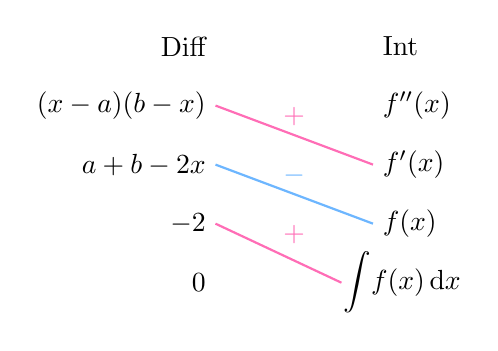
\begin{tikzpicture}[yscale=0.75]
      \draw (-1, 1) node[left]{Diff};
      \draw (1,  1) node[right]{Int};
      \draw (-1, -0) node[left]{$(x - a)(b - x)$};
      \draw (1,  -0) node[right]{$f''(x)$};
      \draw (-1, -1) node[left]{$a + b - 2x$};
      \draw (-1, -2) node[left]{$-2$};
      \draw (-1, -3) node[left]{$0$};
      \draw (1,  -1) node[right]{$f'(x)$};
      \draw (1,  -2) node[right]{$f(x)$};
      \draw (0.5,  -3) node[right]{$\ds\int\!f(x)\,\text{d}x$};
      \draw[thick, M4, -] (-1, -0)--(1, -1); \draw[M4] (0, -0.5) node[above]{$+$};
      \draw[thick, C4, -] (-1, -1)--(1, -2); \draw[C4] (0, -1.5) node[above]{$-$};
      \draw[thick, M4, -] (-1, -2)--(0.6, -3); \draw[M4] (0, -2.5) node[above]{$+$};
    \end{tikzpicture}
  \end{minipage}
  \hspace{5mm}
  \begin{minipage}{0.65\textwidth}
    $\ds\int(x-a)(b-x)\,f''(x)\,\mathrm{d}x \\= \big((x - a)(b - x)\,f'(x) - (a + b - 2 x)\,f(x)\big) - 2\int\!f(x)\,\mathrm{d}x$
  \end{minipage}
\end{sol}

\begin{prp}
  令 $\ds F(x) = \int_{v(x)}^{u(x)} f(\tau)\,\mathrm{d}\tau$, 則 $\ds F'(x) = f(u(x))\cdot u'(x) - f(v(x))\cdot v'(x)$. 
\end{prp}

\begin{prf}
  令 $a\in\mathbb{R}$, $\ds F(x) = \int_{v(x)}^{u(x)} f(\tau)\,\mathrm{d}\tau = \int_{a}^{u(x)} f(\tau)\,\mathrm{d}\tau - \int_{a}^{v(x)} f(\tau)\,\mathrm{d}\tau$. 令 $\ds G(x)\equiv\int_a^x f(\tau)\,\mathrm{d}\tau$, 則 $\ds G'(x) = f(x)$, $\ds F(x) = \int_{a}^{u(x)} f(\tau)\,\mathrm{d}\tau - \int_{a}^{v(x)} f(\tau)\,\mathrm{d}\tau = G(u(x)) - G(v(x))$; 故 $\ds F'(x) = (G(u(x)) - G(v(x)))' = G'(u(x))\cdot u'(x) - G'(v(x))\cdot v'(x) = f(u(x))\cdot u'(x) - f(v(x))\cdot v'(x)$.   
\end{prf}

\begin{ex} 
  \begin{enumerate}\setlength{\itemsep}{0pt}
    \item[]
    \item $\ds F(x) = \int_1^x\frac{1}{1 + \tau^4}\,\mathrm{d}\tau \ie F'(x) = \frac{1}{1 + x^4}$ 
    \item $\ds F(x) = \int_{x}^{2x}\tau^3\,\mathrm{d}\tau \ie F'(x) = (2x)^3\cdot 2 - x^3\cdot 1 = 15x^3$
  \end{enumerate}
\end{ex}

\section*{積分技巧: 部份分式}

\begin{ex}
  若 $a\ne 0$, 求 $\ds\int\!\frac{1}{x^2 - a^2}\,\text{d}x$. 
\end{ex}

\begin{sol}
  由 $\ds\frac{1}{x^2 - a^2} = \frac{1}{2a}\bigg(\frac{1}{x - a} - \frac{1}{x + a}\bigg)$, $\ds\int\!\frac{1}{x^2 - a^2}\,\text{d}x = \int\frac{1}{2a}\bigg(\frac{1}{x - a} - \frac{1}{x + a}\bigg)\,\text{d}x = \frac{1}{2a}\big(\ln|x - a| - \ln|x + a|\big)$
\end{sol}

\begin{ex}
  求 $\ds\int\!\frac{x}{x^2 - 5x + 6}\,\text{d}x$. 
\end{ex}

\begin{sol}
  $\ds\frac{x}{x^2 - 5x + 6} = \frac{x}{(x - 3)(x - 2)} = \frac{A}{x - 3} + \frac{B}{x - 2} \ie x = A\,(x - 2) + B\,(x - 3)$. 代入 $x = 3\ie 3 = A$; 代入 $x = 2\ie 2 = B(2 - 3) \ie B = -2$, 故 $\ds\frac{x}{x^2 - 5x + 6} = \frac{3}{x - 3} - \frac{2}{x - 2}$, $\ds\int\!\frac{x}{x^2 - 5x + 6}\,\text{d}x = \int\bigg(\frac{3}{x - 3} - \frac{2}{x - 2}\bigg)\,\text{d}x = 3\ln|x - 3| - 2\ln|x - 2|$
\end{sol}

\end{document}
